\chapter{Event Selection}
\label{ch:selection}

%Two analysis methods are pursued to select samples that can be 
%used to extract the signal yield from the data in an optimal way.
The resonances in search decay to two SM Higgs bosons. However, Higgs bosons further decay almost immediately. Therefore, it is critical to reconstruct Higgs bosons decay products with the high precision. 

\section{Higgs and Z Boson Selection}



Only dilepton pairs having net charge of zero are considered as \ZtoLL~ candidates. 
Pairs of prompt isolated leptons must have a dilepton mass greater than 76 GeV. This ensures the orthogonality with HIG-17-006 bbVV analysis (later also referred to as bbWW analysis) as well as helps selecting decays of real Z bosons.

Higgs boson candidates are reconstructed from the b jet pairs utilising the two b jets with the highest CMVAv2 discriminant value. We do not veto additional b jets as with the increased PU growths the probability to have more b jets. 

Double Higgs boson candidate is computed as a sum of Lorentz vectors of the \ZtoLL~ candidate, MET, and a \HBB~ candidate. Then, we compute the transverse mass of that object. 

This transverse mass definition that we follow is one of the commonly used and is logical in the sense that we subtract the longitudinal momentum component which leaves us with the transverse momentum components only (while the energy remains the total energy). More precisely, as the z-component of the neutrinos' momentum is unknown and we decided not to reconstruct it, we form a pseudo transverse mass: $\tilde{M}_T(HH) = \sqrt{E^2 - p_{z}^2}$ (further referred as transverse mass for brevity), where $E$ and $p_z$ are the energy and the z-axis component of the Lorentz energy-momentum vector of the HH candidate.

The resulting distribution, $\tilde{M}_T(HH)$, is what will be used in the binned shape analysis with the Higgs Combination Tool following the section "Binned shape analysis" as described at the twiki page~\cite{CombinedLimit}. Shape analysis is more sensitive than the simple cut-and-count experiment (one bin distributions) since more information/discrimination power is given to the likelihood function. 

%:
%\begin{center}
%    \small{\texttt{https://twiki.cern.ch/twiki/bin/view/CMS/SWGuideHiggsAnalysisCombinedLimit}}
%\end{center}
Initial data files, called ntuples, have enormous size of the order of more than a Terabyte per background process. To reduce the size of the ntuples and remove clear background events (on the other hand, to remove signal-like events we apply a sophisticated selection and use a BDT), we apply a "common-sense" HH preselection, which starts with the requirement on dilepton mass to be greater than 50 GeV and the event to contain at least two "good" jets - with $p_{T} > 30$ GeV and $|\eta| < 2.4$. In addition to requirements on Higgs bosons decaying to b quarks mentioned above, we define Z bosons as two opposite sign muons with $p_{T} > 20/15$ GeV (leading/subleading lepton) or two opposite sign electrons with $p_{T} > 25/15$ GeV (leading/subleading lepton). 



Later analysis cuts, the selection chain to improve signal-background separation, include: 

 \begin{itemize}
 \item  the requirement of at least two b jets in the event, out of which two with the highest CMVAv2 score are used to define \HBB ~candidate
 \item  the lower end cut on the \HBB ~mass set to 20 GeV to remove the low mass resonances, while giving BDT as many events in the CRDY as possible at the same time. The upper end cut is not explicitly set for the same purpose. The actual \HBB ~mass distribution after the analysis selection is concentrated in the range 30 to 220 GeV
 \item  the Z boson selection takes the most energetic two leptons of the opposite sign and requires their dilepton mass to pass 76 GeV < Z mass < 106 GeV condition used for the signal region definition. This is a standard $\pm$ 15 GeV window for Z boson selection whose lower end also preserves othogonality with the existing HIG-17-006 bbVV analysis
 \item  HH candidate is approximated by the sum of \ETslash, Z, and \HBB~decays. A loose cut on HH transverse  $>100$ GeV removes evidently background events
 \item  finally, an additional set of \ETslash cuts is used to ensure orthogonality with the existing HIG-18-013 bbZZ analysis focusing on the 2b jets + 2 leptons + 2 quarks, see Table \ref{metCuts}. The MET cuts have been optimised by both analyses to yield the best limit when the results of two measurements are combined. 
 \end{itemize}


\begin{table}[H]
\begin{center}
\caption{\ETslash cut to orthogonalise the analysis with respect to HIG-18-013.}
\begin{tabular}{|c|c|} \hline
{Signal mass, GeV} &  \ETslash cut, GeV\\\hline
260-300     &                                \textgreater~40 \\
350-600     &                                \textgreater~75 \\
650-1000    &                                \textgreater~100 \\
\hline
\end{tabular}
\label{metCuts}
\end{center}
\end{table}


\begin{figure}[H]%hbpt?                                                                       
  \begin{center}
    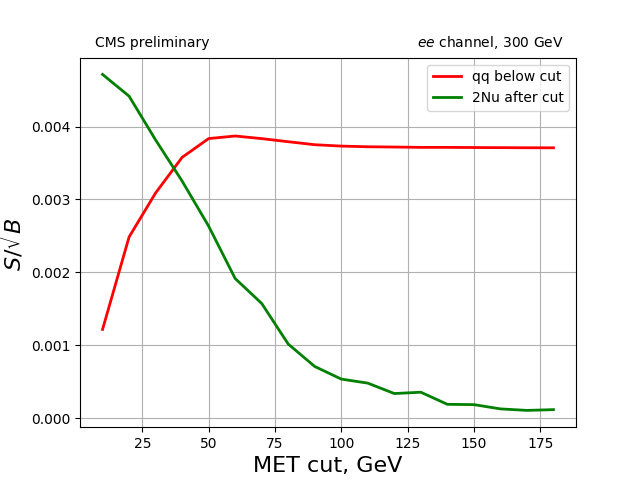
\includegraphics[width=0.45\textwidth]{ee_300_met.png}
    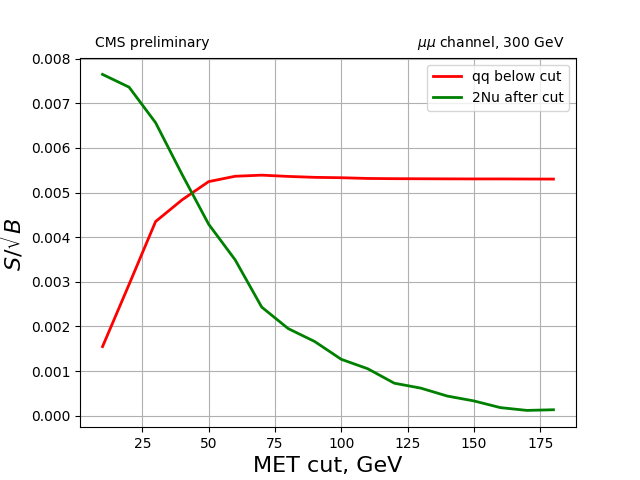
\includegraphics[width=0.45\textwidth]{mm_300_met.png}\\
    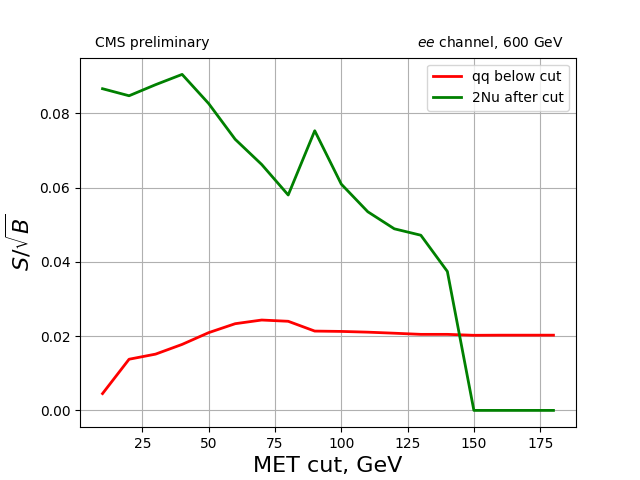
\includegraphics[width=0.45\textwidth]{ee_600_met.png}
    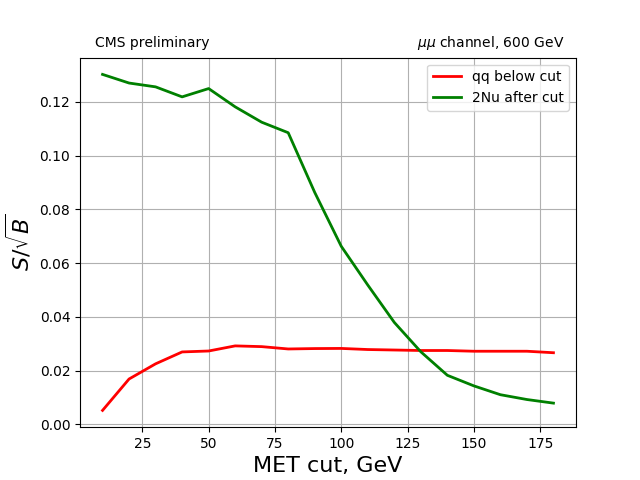
\includegraphics[width=0.45\textwidth]{mm_600_met.png}\\
    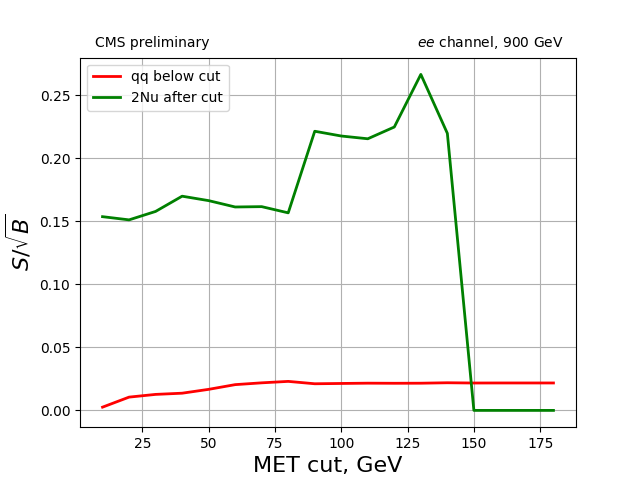
\includegraphics[width=0.45\textwidth]{ee_900_met.png}
    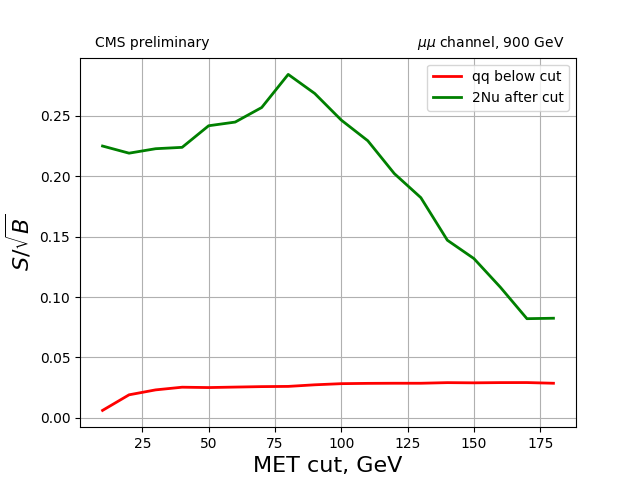
\includegraphics[width=0.45\textwidth]{mm_900_met.png}\\
    \caption{ Significance-like ($\sqrt{S}/B$) figure of merit as a function of the MET cut. Green curve shows the significance for our analysis keepings event above the cut, red curve is for HIG-18-013 analysis and their phase space is below the cut value. Top: 300 GeV cut. Middle: 600 GeV cut. Bottom: 900 GeV cut. On the left dielectron channel is shown, while dimuon plots are on the right. }
    \label{fig:met_cuts}
  \end{center}
\end{figure}




\section{\HBB ~and \ZtoLL ~variables to define signal and control regions}

In this analysis we define three regions in the \HBB ~and \ZtoLL
~space. Two regions, CRDY and CRTT, are used to extract the
normalizations of DY and \ttbar backgrounds correspondingly. Signal region (Fig. ~\ref{fig:regions}) is chosen by
the set of \HBB~and \ZtoLL ~cuts \ref{fig:regions}. To further reduce background contamination in this region, an additional cut on the MVA output is used. Boosted decision trees (BDT) MVA technique is employed to
separate background from signal. Below we describe in details
selection of each region and BDT construction. 

%% Skimming is applied
%% before building BDT to remove unnecessary background, while still
%% keeping a lot of events for BDT training. The set of "HH loose
%% common-sense" \label{hhSelection} skimming/preselection cuts includes: Dilepton (ee/mm)
%% mass $>$ 50 GeV, 2 or more jets: pt $>$ 30 GeV and $|\eta| < 2.4GeV$. Then, we
%% select two or more b-jets, \HBB~ mass should be greater than 20 GeV,
%% exactly two leptons, dilepton mass higher than 76 GeV, transverse mass
%% of HH higher than 100 GeV. The definition of the signal and control regions is illustrated in Fig. \ref{fig:regions}. The signal region is selected in the range of
%% 76 $<$ \mll~ $<$ 106 GeV and %75 $<$ \mbb~ $<$ 175 GeV. This corresponds to the
%% 90 $<$ \mbb~ $<$ 150 GeV. This corresponds to the
%% Z mass +- 15 GeV window. OA
For CRDY we invert \HBB ~cut, keeping in the lower sideband only events
with the mass of Higgs boson higher than 20 GeV to avoid fakes from
QCD. For CRTT we invert \ZtoLL ~cut, keeping only high mass sideband to
ensure the orthogonality with the existing HIG-17-006 bbVV analysis, since the lower sideband is already included in the phase space used by them. 


\begin{figure}[!htb]%hbpt?                                                                       
  \begin{center}
    %\raisebox{0.17\height}                                                                     
    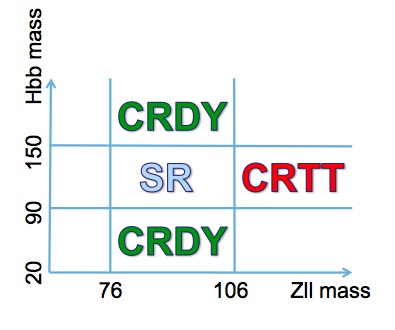
\includegraphics[width=0.45\textwidth]{regions.png}
    \caption{ Signal region, control region \ttbar, and control region Drell-Yan in the phase space of \ZtoLL \ ~and ~\HBB ~masses.    }
    \label{fig:regions}
  \end{center}
\end{figure}


%% \begin{table}
%% \begin{center}
%% \caption{Efficiency of the BDT selection requirement. Dielectron channel. Left: 300 GeV signal mass hypothesis. Right: 900 GeV case.}
%% \begin{tabular}{|c|c|c|} \hline
%% {Process} &  Efficiency at 300 GeV, \% &  Efficiency at 900 GeV, \% \\\hline

%% signal (bbZZ) &                       85 &                       86 \\
%% signal (bbWW) &                       60 &                       82 \\
%% \ttbar        &                       28 &                       $\sim$ 0 \\
%% Drell-Yan     &                       64 &                       $\sim$ 0 \\
%% Single top    &                       33 &                        1 \\
%% ZH            &                       76 &                        4 \\
%% Dibosons      &                       76 &                        2 \\\hline

%% \end{tabular}
%% \label{EfficiencyBDT}
%% \end{center}
%% \end{table}


\begin{table}                                                                                                                                                                          
\begin{center}      
                                                                                                                                                                   
\caption{Efficiency of the BDT selection requirement. $ee$ channel (top) and $\mu\mu$ channel (bottom). }
\begin{tabular}{|c|c|c|}
\hline
sample & Efficiency at 300 GeV, [\%] &  Efficiency at 900 GeV, [\%] \\
\hline
signal (bbZZ) &                        89.2 &                        94.9 \\
signal (bbWW) &                        75.0 &                        88.4 \\
\ttbar        &                        28.8 &                         0.2 \\
Drell-Yan     &                        74.2 &                         1.2 \\
Single top    &                        33.1 &                         1.1 \\
ZH            &                        88.8 &                        10.7 \\
Dibosons      &                        90.0 &                         5.0 \\
\hline
\end{tabular}
%\vspace*{1cm}
\begin{tabular}{|c|c|c|}
\hline
sample &  Efficiency at 300 GeV, [\%] &  Efficiency at 900 GeV, [\%] \\
\hline
signal (bbZZ) &                        58.1 &                        91.1 \\
signal (bbWW) &                        25.9 &                        96.3 \\
\ttbar        &                        13.6 &                         0.2 \\
Drell-Yan     &                        39.0 &                         0.8 \\
Single top    &                        13.0 &                         0.2 \\
ZH            &                        56.0 &                         8.4 \\
Dibosons      &                        51.4 &                         6.2 \\
\hline
\end{tabular}

\label{EfficiencyBDT}                                                                                                                                                                  
\end{center}                                                                                                                                                                           
\end{table} 


%
%
%\begin{figure}[tbp]
%  \begin{center}
%    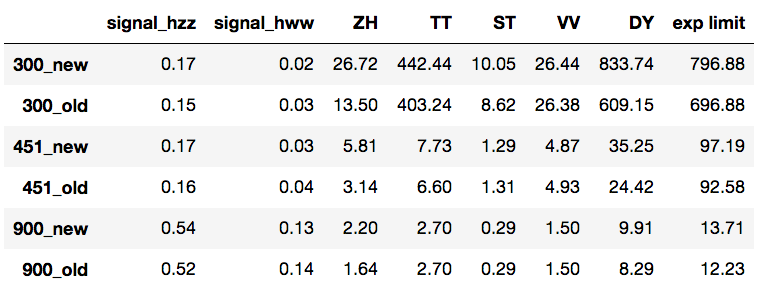
\includegraphics[width=0.91\textwidth]{ee_yields.png}
%    \caption{Yields for ee channel before and after the tight isolation bug fix in the HEPPY. The effect is minimal as can be seen in the final limit. }
%    \label{fig:yields_ee}
%  \end{center}
%\end{figure}
%


\section{Signal and background characteristics}

The signal region is further purified removing backgrounds by applying the cut on the BDT
output (Table ~\ref{EfficiencyBDT} contains the efficiency numbers for the BDT cut). 
The first set of BDT variables in the early version of the analysis included 30-50 variables, which could potentially discriminate signal from the background. The set contained variables related to the kinematic properties of the signature, as well as a dozen of angular variables. After the first optimization of the BDT training and produced ranking of variables, nine best variables were determined and chosen to be used for the final analysis. Removal or addition of other variables did not improve the performance significantly. To simplify the analysis, the same set of nine variables is used in both low and high mass trainings and for both spin hypotheses.

With 16 masses points in the range from 250 to 1000 GeV, one can: train 16 discriminants, train one complex hyperparametrised neural network, split the mass range into regions with the similar kinematics and thus train only few BDTs. The latter is the approach that has been adopted by mature (legacy) HH analyses, and we are following the same procedure. We split the mass range into two: low mass and high mass (\`a la HIG-17-002 and HIG-17-008). These simplification costs some performance loss but allows analysis to proceed with just two BDTs instead of training one BDT per mass point, which would require more than a dozen of trainings per heavy resonance. In case of the infinite statistics, training a dedicated BDT for each
signal mass hypothesis would give a better performance, but in our case we are statistics dominated, thus training only two BDTs also has benefits in terms of the size of the signal sample, absence of the overtraining etc. In addition, the adopted path saves computational resources. Lastly, physics-wise, bbZZ signature is not the most sensitive, bb$\gamma$$\gamma$ is due to an excellent CMS diphoton mass resolution. Thus, the difference in sensitivity is a factor of 30-100 depending on the mass. Therefore, training a dozen of BDTs is clearly impractical. For more discussion on the topic please refer to the chapter \ref{ch:BDT}.





%In addition, it would require a training of 16 BDTs per particle (BulkGraviton in our case). 
The low/high mass boundary value for HH analyses is chosen typically in the range 300-450
GeV. In our case the performance of the boundary around 300 GeV (area under the ROC curve
for low mass BDT is 0.9138 and 0.9805 for high mass BDT) is
similar to the boundary option at the 450 GeV (area under the ROC curve
for low mass BDT is 0.9086 and 0.9957 for high mass BDT), and to the one in the
middle of the range (area under the ROC curve
for 400 GeV for low mass BDT is 0.9074 and 0.9928 for high mass BDT). 
%https://indico.cern.ch/event/628835/contributions/2639777/attachments/1483653/2302207/Rami_HH_27June2017_v3.pdf
Therefore, we chose the value of 450 GeV, which
is also a choice of the bbbb analysis \cite{bbbb}. Upon running the full analysis chain up to the expected limits, the choice of 450 GeV was verified to be the best split point option: the usage of the high mass BDT at the 400 GeV or low mass BDT at the 500 GeV was yielding suboptimal results thus confirming the mass boundary choice. 

Splitting the mass range into two regions, we arrive at the low
mass BDT, which merges (with the weight '1') seven signal samples:
250, 260, 270, 300, 350 400, 450 GeV, and the high mass BDT, which combines nine signal samples of 
masses: 500, 550, 600, 650, 700, 750, 800, 900, 1000. In each case the
composition of the background is the same, it is a mix (by cross
section) of \ttbar and Drell-Yan plus jets.


Cut flow for $ee$ and $\mu\mu$ channels from the generator level up to before the BDT selection is shown on the figures ~\ref{fig:cutFlow}. In the cut flow table ~\ref{fig:cutFlow} the following definitions are used: very loose selection means all GsfElectrons and Muons from the basic collections that match generator level electrons/muons and pass the very minimal kinematic cuts; loose selection means loose POG selection consisting of kinematic cuts, impact parameters dxy and dz, and iso cuts. Shown final efficiency values are given in terms of the number of events ~\ref{cutFlowEvents}:

\begin{table}
\begin{center}
\caption{Number of events surviving analysis cuts corresponding to the last entry in the ~\ref{fig:cutFlow} .}
\begin{tabular}{|c|c|c|} \hline
{Process, mass point} &  ee channel, \% &  mm channel, \% \\\hline
bbZZ, 300 GeV &                    2256     &                    4511 \\
bbWW, 300 GeV &                    53       &                    85 \\
bbZZ, 900 GeV &                    8034     &                    12963 \\
bbWW, 900 GeV &                    12       &                    23 \\\hline
\end{tabular}
\label{cutFlowEvents}
\end{center}
\end{table}



\section{Data and MC comparison\label{sec:compareDataMC}}
%Signal region BDT sideband plots as well as unblind signal region plots show good data-MC agreements.
BDT selection is applied in the signal region only, we are not cutting on BDT for control regions, therefore, all the mass
points belonging to the low mass region (and separately to the high mass region) have the same background and data distributions. Thus, we provide plots for two mass points: one mass point representing low mass region, 300 GeV, and one mass point representing high mass region, 900 GeV. 
% for other pass point only signal distribution will change,
%however, data/background comparison and their ratio will not. At the same time, BDT outputs are mass point specific, because are trained for two different mass regions - low and high mass regions, and are evaluated for each mass point separately. Thus, we show all the BDT plots. 
Signal bbZZ and bbWW rates for all plots are multiplied additionally by a factor of 500 purely for the visualization purpose and do not go in the real analysis. 

%Prefit plots are available in the Appendix ~\ref{sec:datamc}. Control regions only postfit plots have been produced during an extensive discussion with Higgs conveners at HyperNews, and it was shows that upon inclusion of the SR in the fit the data-MC agreement is slightly better. 

Postfit plots that include SR in the simultaneous fit with control regions, hence a common jargon name "Full postfit" plots, in contrast to the control regions only type of the fit, or a control regions plus signal region sideband. Figures ~\ref{fig:MCcomparisons} - ~\ref{fig:MCcomparisons_radion} show data and MC comparison in the SR, CRDY, and CRTT. For both $ee$ and $\mu\mu$ channels, low and high mass regions. The latest style plots produced for the analysis public document (Physics Analysis Summary called "PAS") can be found at Fig.~\ref{fig:MCcomparisons} for the graviton case and Fig.~\ref{fig:MCcomparisons_radion} for the radion case. 


%%%%%%%%%%%%%%%%%%%%%%%%%%%%%%%%%%%
%%%%%%%%%%%%%%%%%%%%%%%%%%%%%%%%%%%

Distributions of nine variables that go into the BDT have been studied in depth during the pre-approval process and are available in the Appendix of the analysis note ~\cite{bbZZAN}. All variables show good data/MC agreement after applying postfit scale factors (not to be confused with the POG recommended scale factors in the section below). %After the tight isolation cut fix in the HEPPY framework the results/shapes are almost unchanged (it is also can be observed from the table of yields ~\ref{fig:yields_ee}).  At the yields table ~\ref{fig:yields_ee}, 450 GeV mass point, since evaluated using the high mass BDT, is called 451 GeV for clarity purposes. 
The most important variables in this analysis, namely the BDT itself and the variable that we fit, \mTHH, are shown in the Fig.~\ref{fig:MCcomparisons} for graviton and in Fig.~\ref{fig:MCcomparisons_radion} for the radion. 


\begin{figure}[tbp]
  \begin{center}
    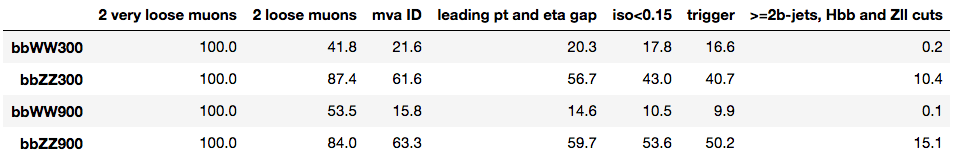
\includegraphics[width=0.91\textwidth]{cutflow_mm.png}\\
    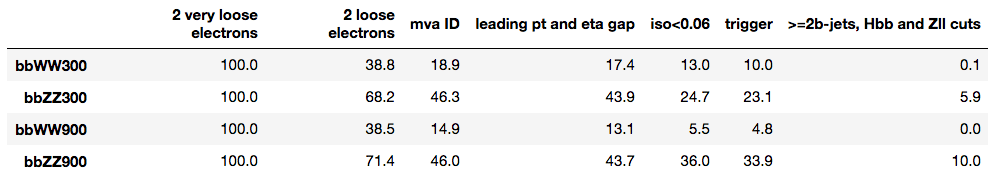
\includegraphics[width=0.91\textwidth]{cutflow_ee.png}\\
    \caption{Cut flow for mm (top) and ee (bottom) channels. }
    \label{fig:cutFlow}
  \end{center}
\end{figure}


                                                                                                                                            

\begin{figure}[tbp]
  \begin{center}
    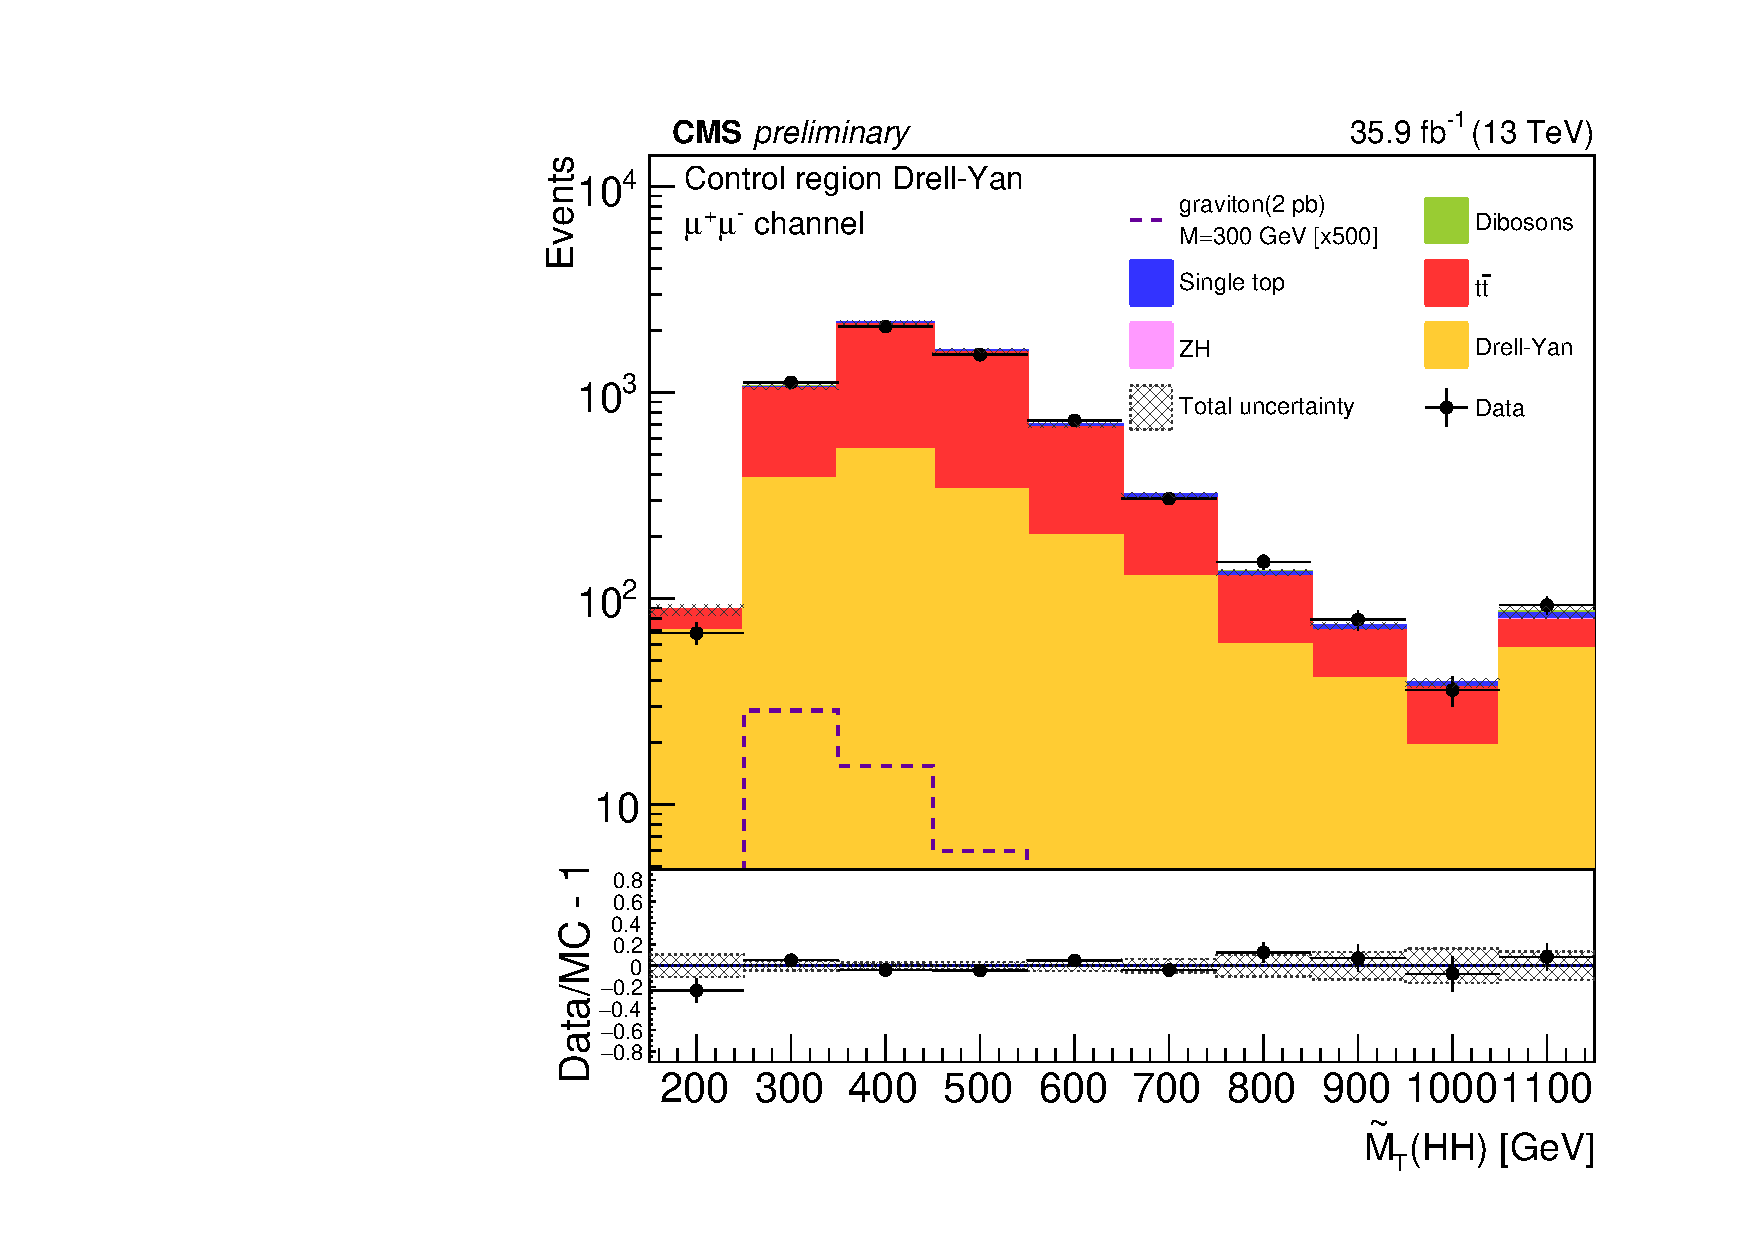
\includegraphics[width=0.31\textwidth]{hhMt_mm_CRDY_FullPostfit_plot_nov16_2_graviton.pdf}
    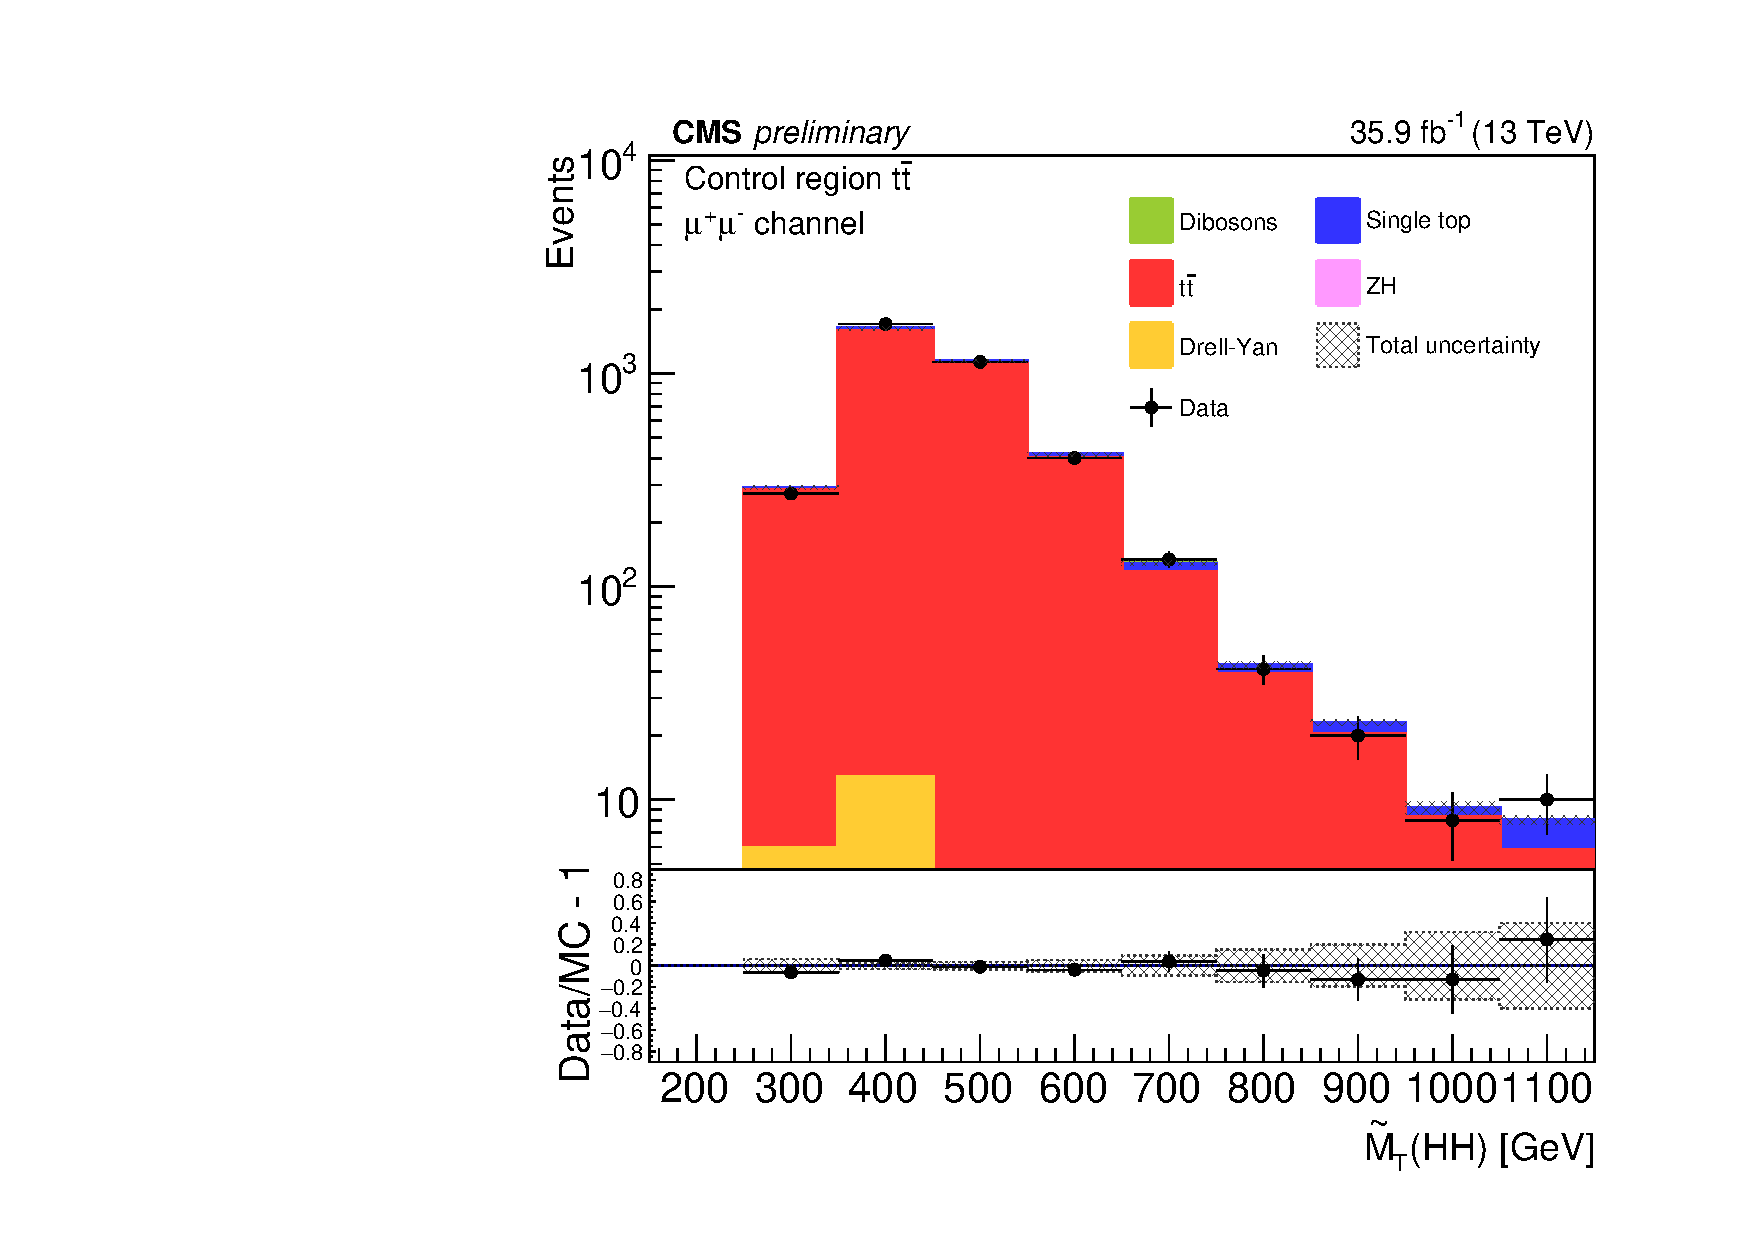
\includegraphics[width=0.31\textwidth]{hhMt_mm_CRTT_FullPostfit_plot_nov16_2_graviton.pdf}
    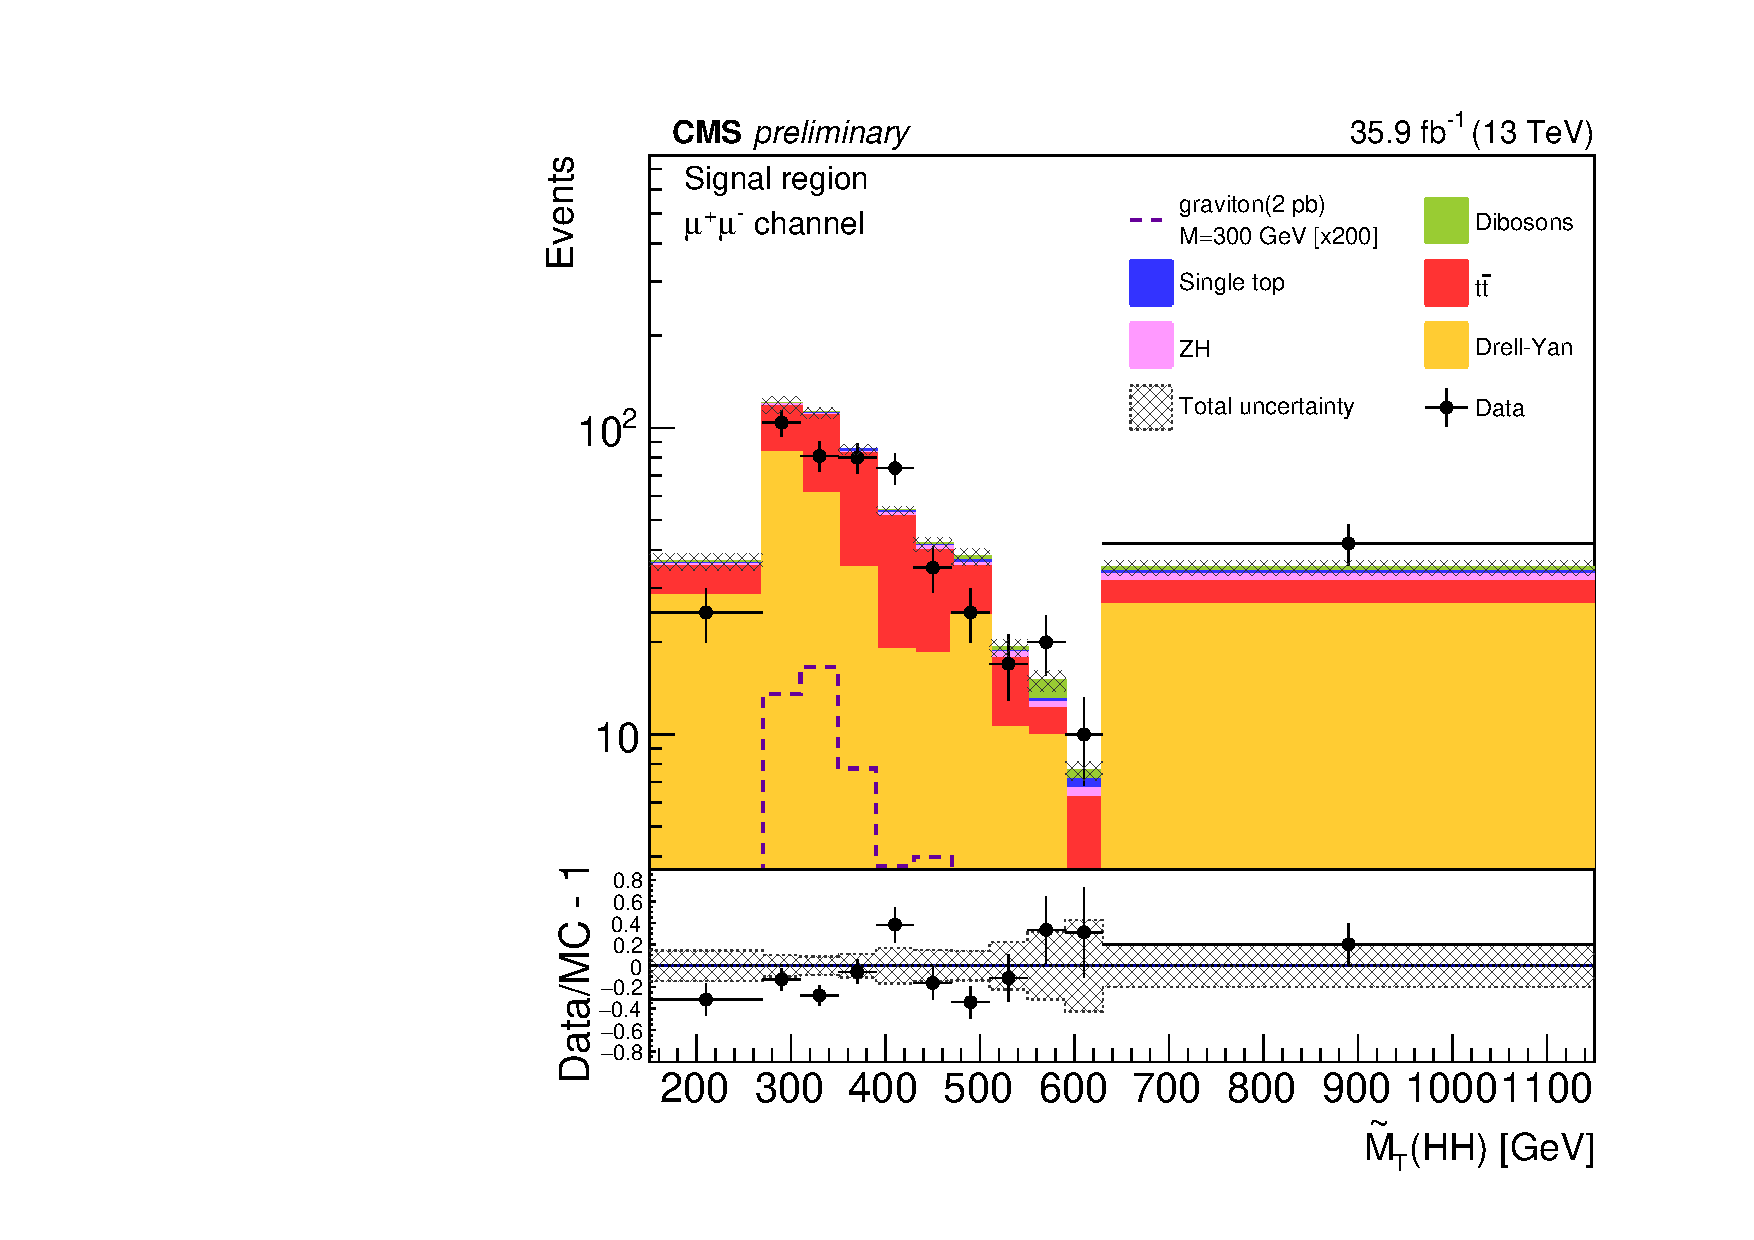
\includegraphics[width=0.31\textwidth]{hhMt_mm_SR_FullPostfit_plot_nov16_2_graviton.pdf} \\
    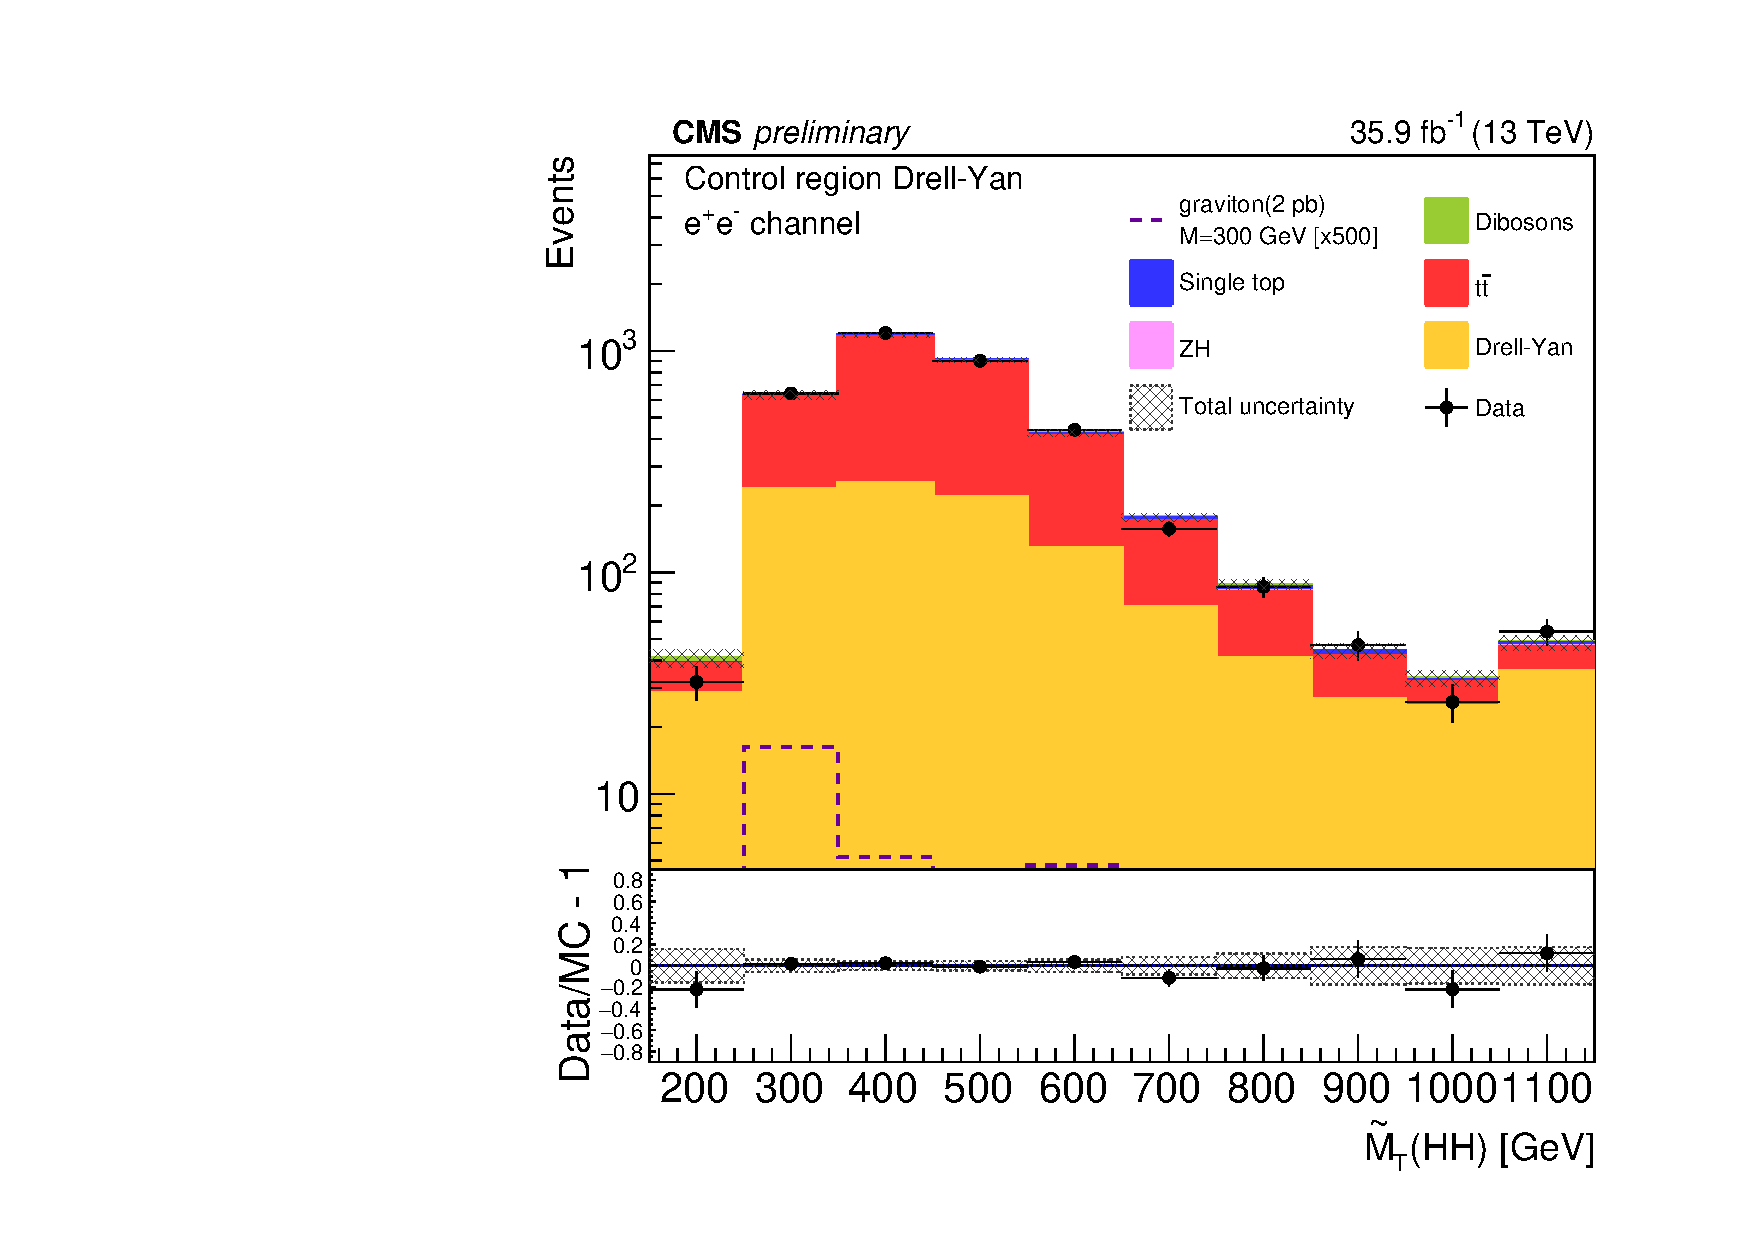
\includegraphics[width=0.31\textwidth]{hhMt_ee_CRDY_FullPostfit_plot_nov16_2_graviton.pdf}
    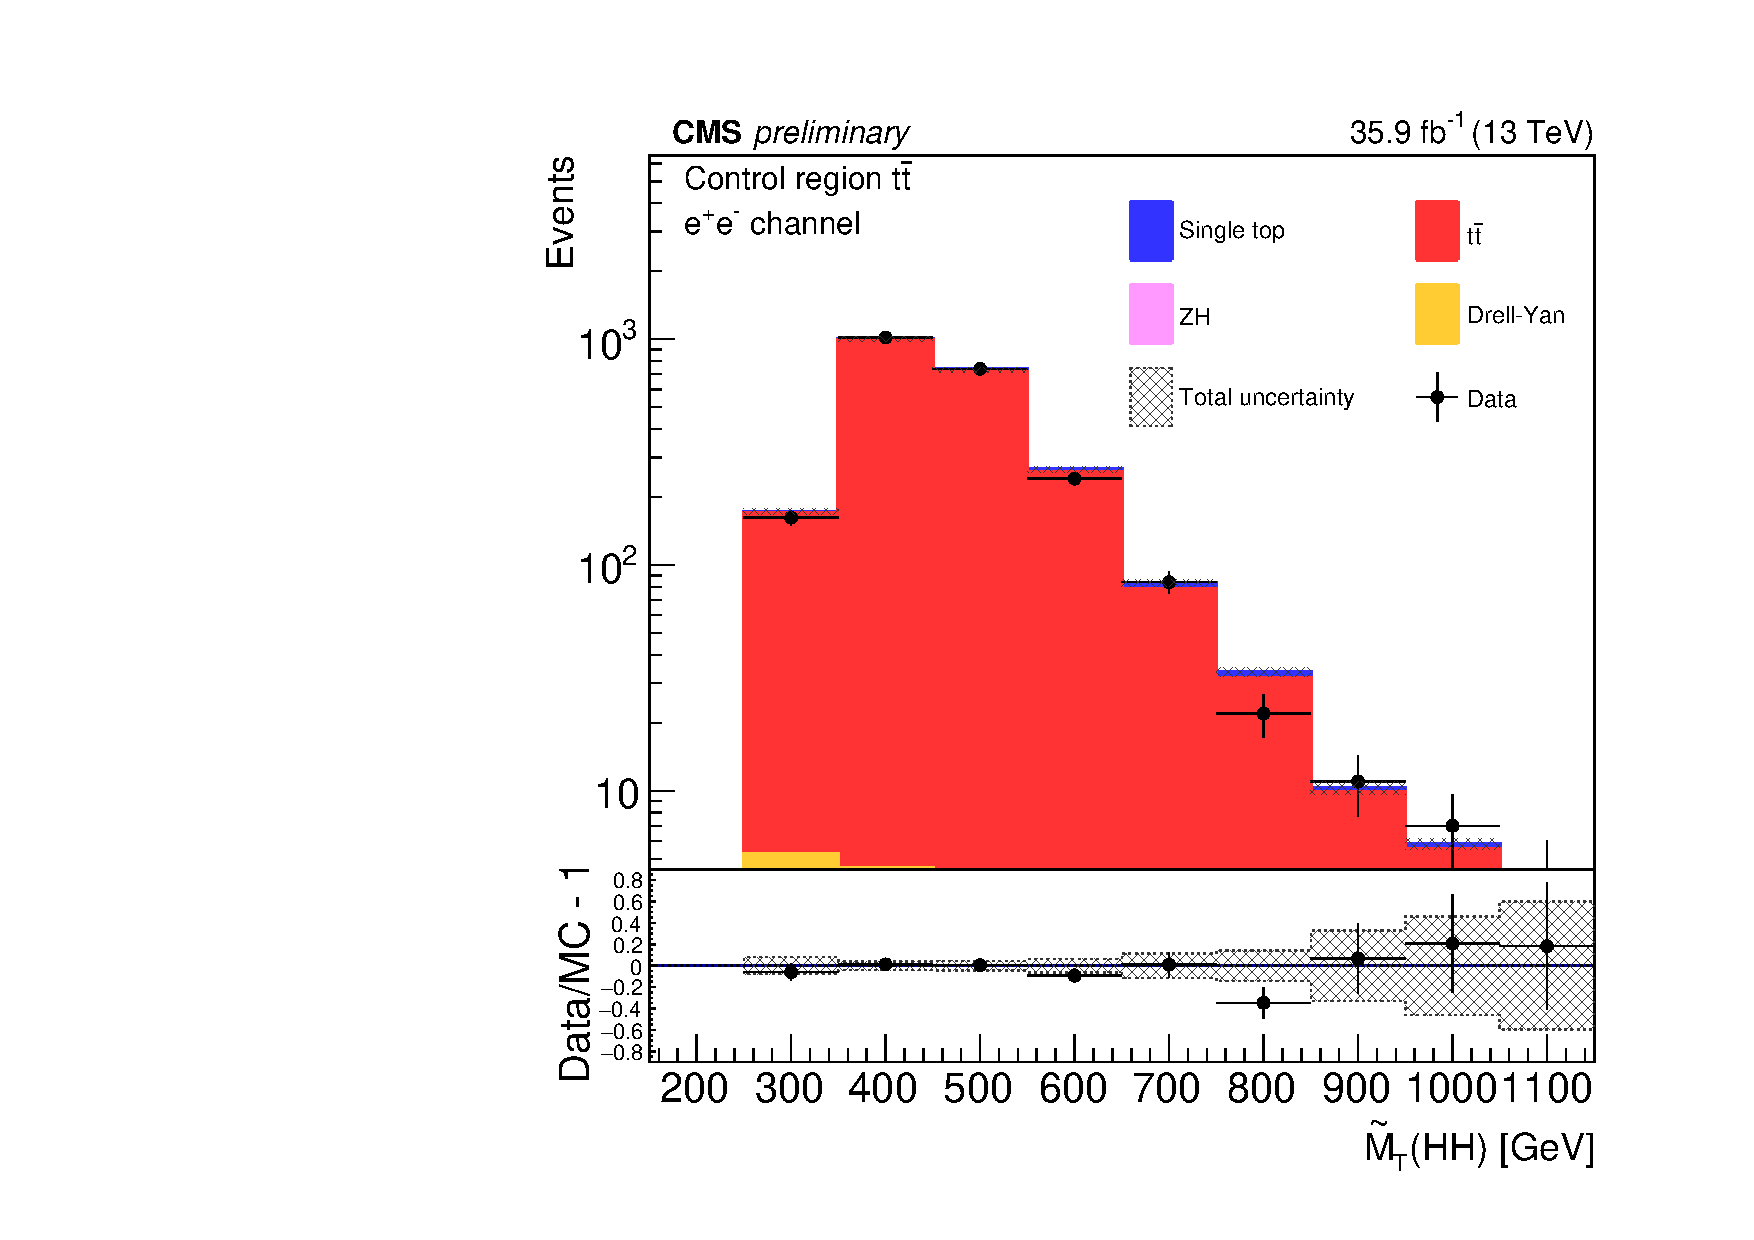
\includegraphics[width=0.31\textwidth]{hhMt_ee_CRTT_FullPostfit_plot_nov16_2_graviton.pdf}
    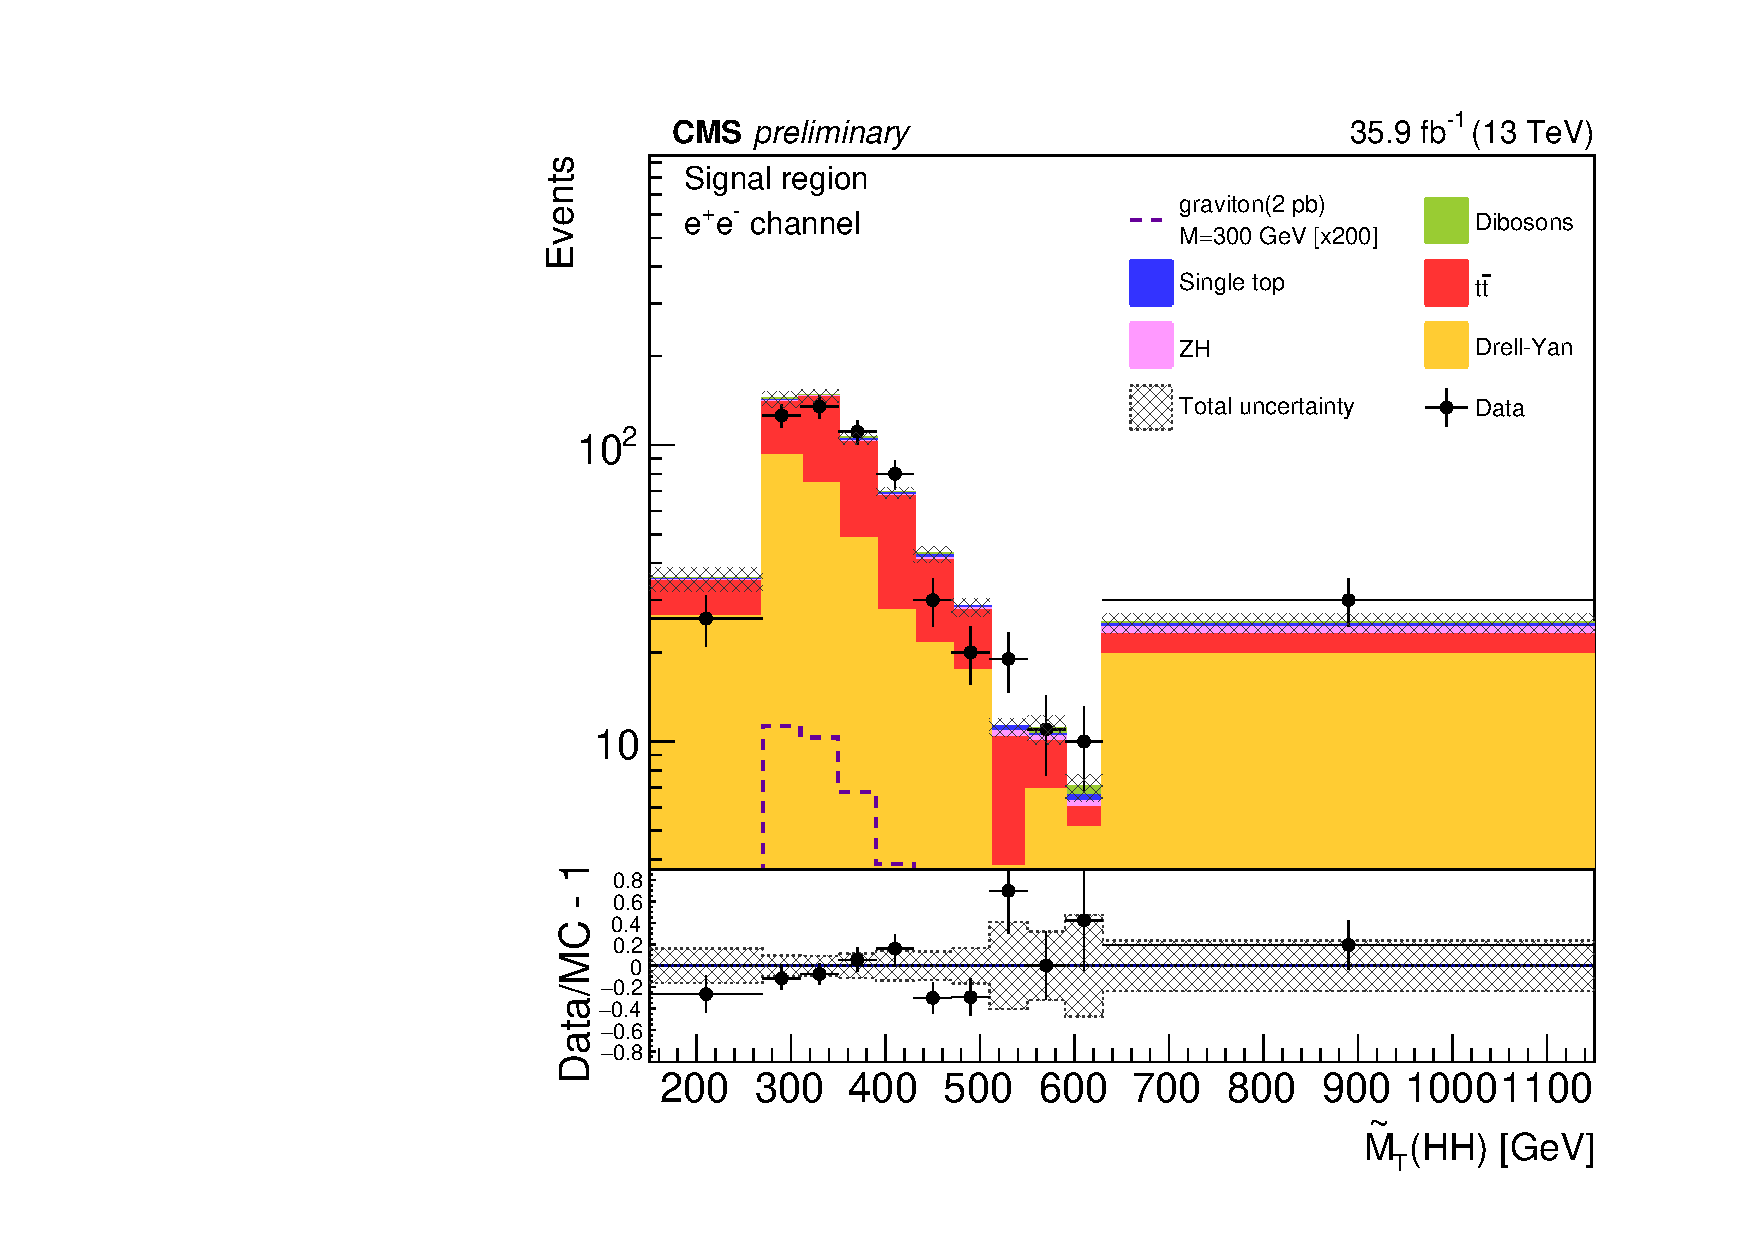
\includegraphics[width=0.31\textwidth]{hhMt_ee_SR_FullPostfit_plot_nov16_2_graviton.pdf}
    \caption{Transverse mass of the reconstructed HH candidates for data, the simulated signal graviton sample
    for the 300 GeV mass hypothesis, and simulated backgrounds scaled according to the fit results. The top
    row shows the figures for the muon channel while the bottom row is for the electron channel. For each row,
    the left plot is for the Drell-Yan control region, the middle is for the \ttbar control region, and the right
    is for the signal region. Signal normalization choice is discussed in the text. The crosshatched area represents
    the sum of statistical and systematic uncertainties.}
    \label{fig:MCcomparisons}
%                                                                                                                 
% Comparison of data and simulation.  Transverse mass of                                                          
%      the reconstructed HH candidate for 300 GeV signal mass                                                     
%      hypothesis, electron channel. Left: Drell-Yan control region. Middle: \ttbar                               
%      control region. Right: signal region. }                                                                    
%    \label{MCcomparisons_electrons}                                                                              
  \end{center}
\end{figure}




\begin{figure}[tbp]
  \begin{center}
    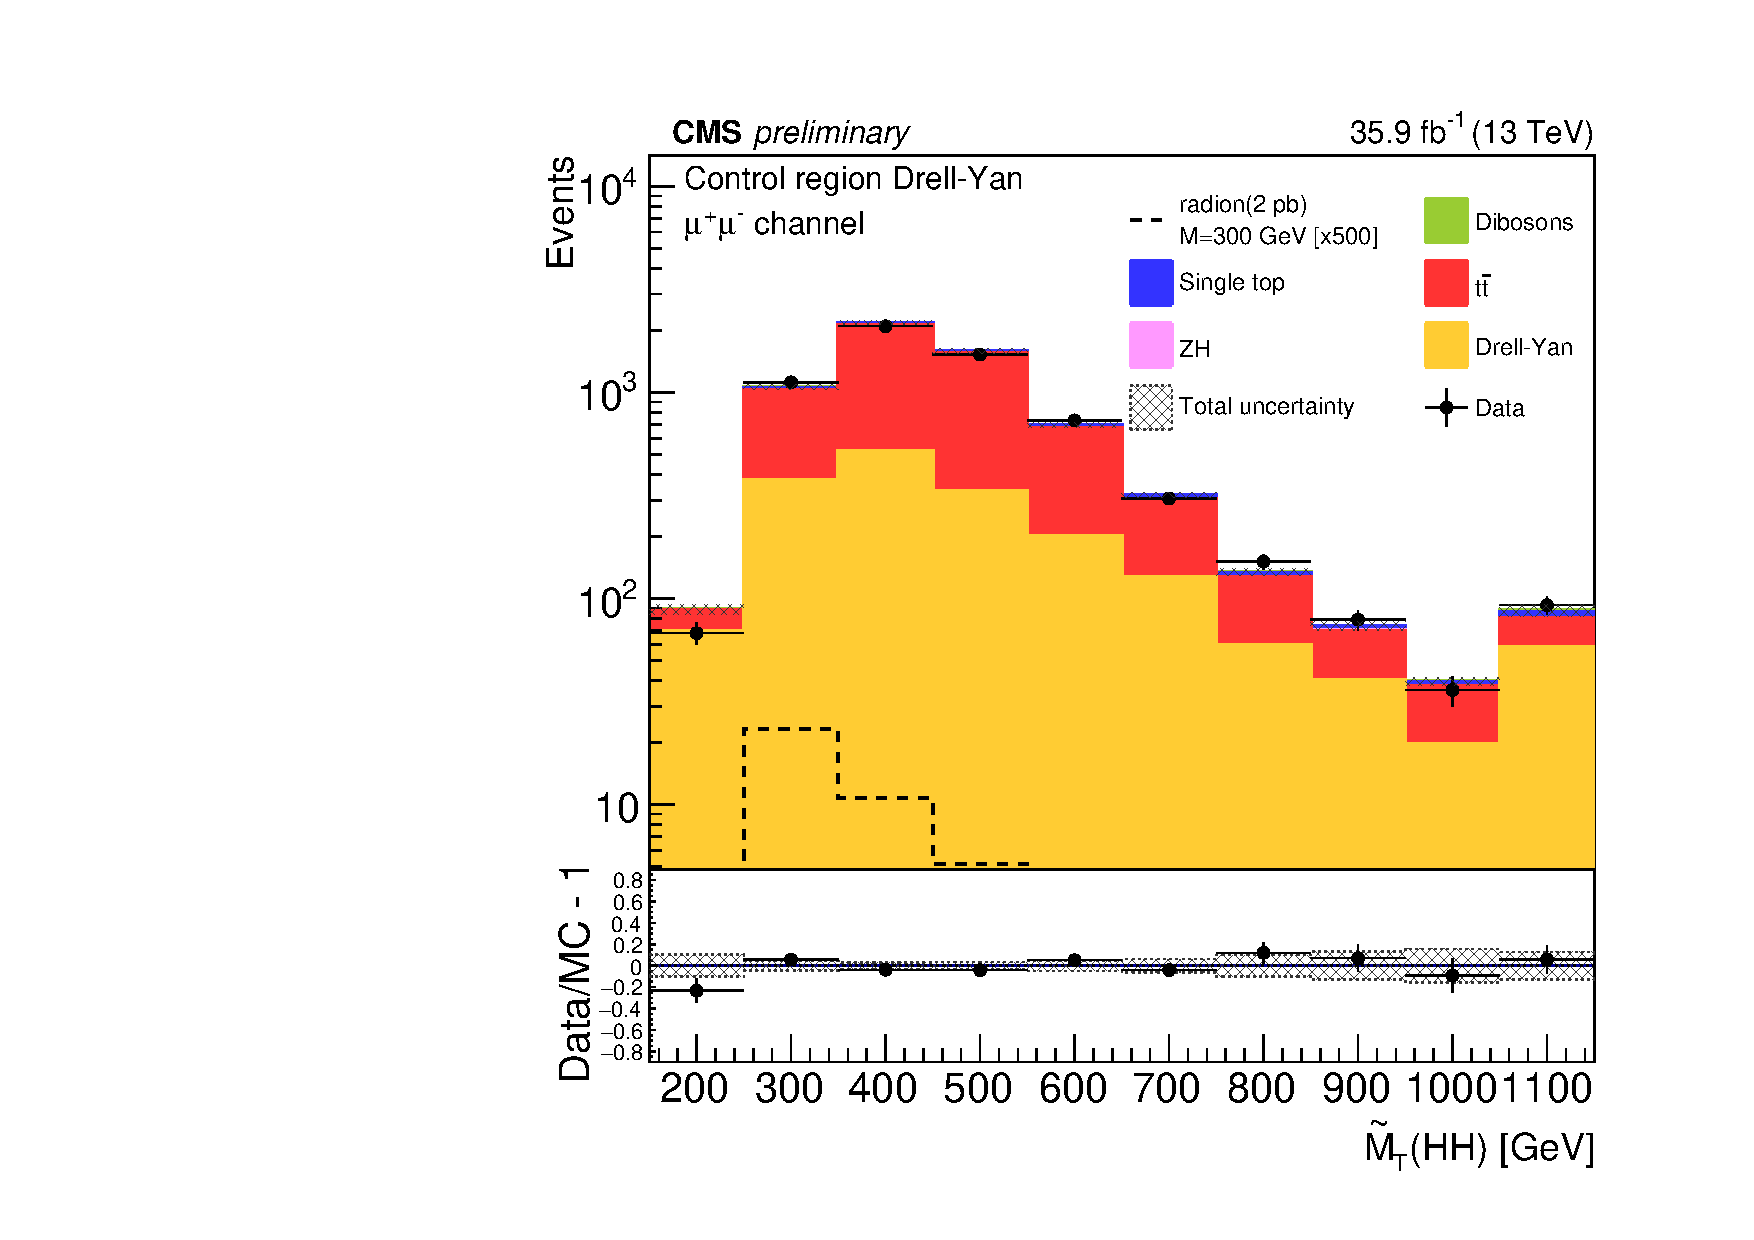
\includegraphics[width=0.31\textwidth]{hhMt_mm_CRDY_FullPostfit_plot_nov16_2_radion.pdf}
    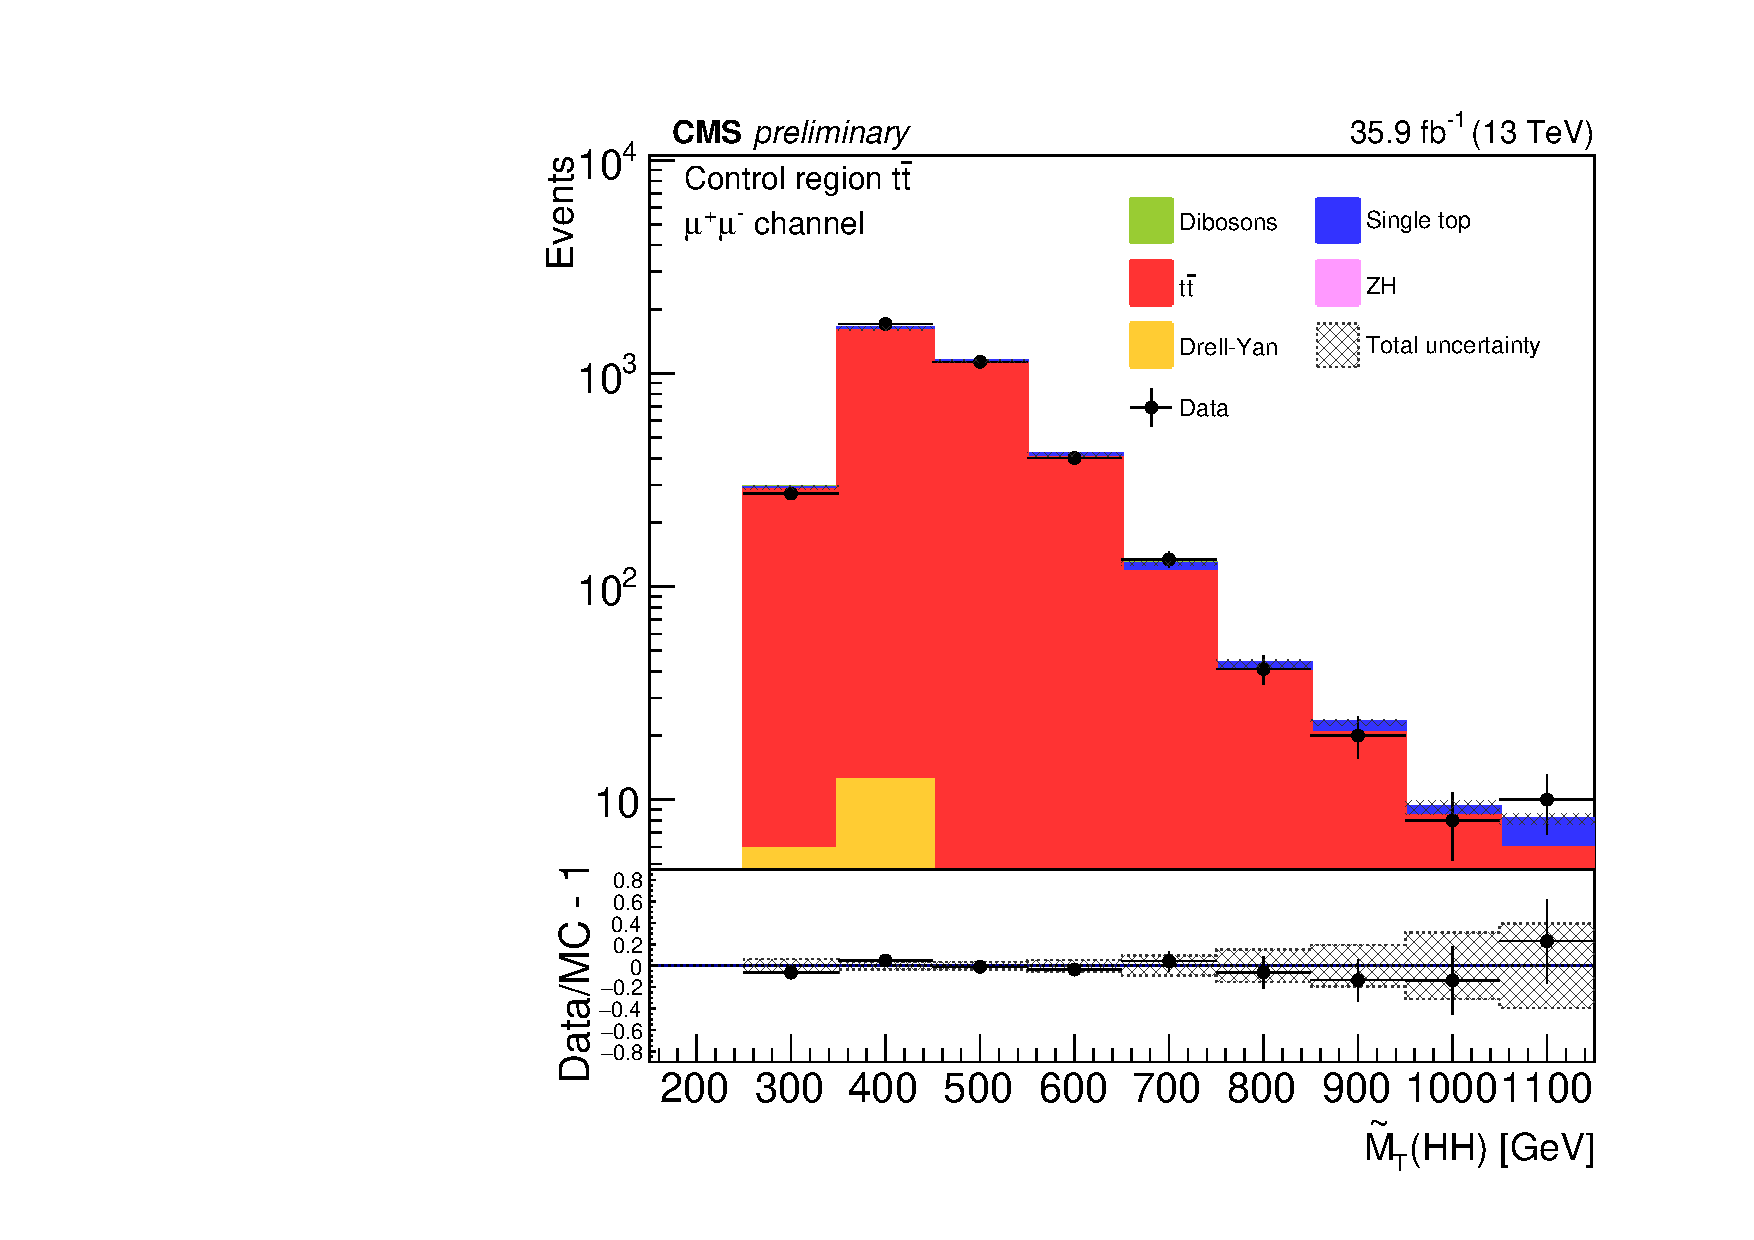
\includegraphics[width=0.31\textwidth]{hhMt_mm_CRTT_FullPostfit_plot_nov16_2_radion.pdf}
    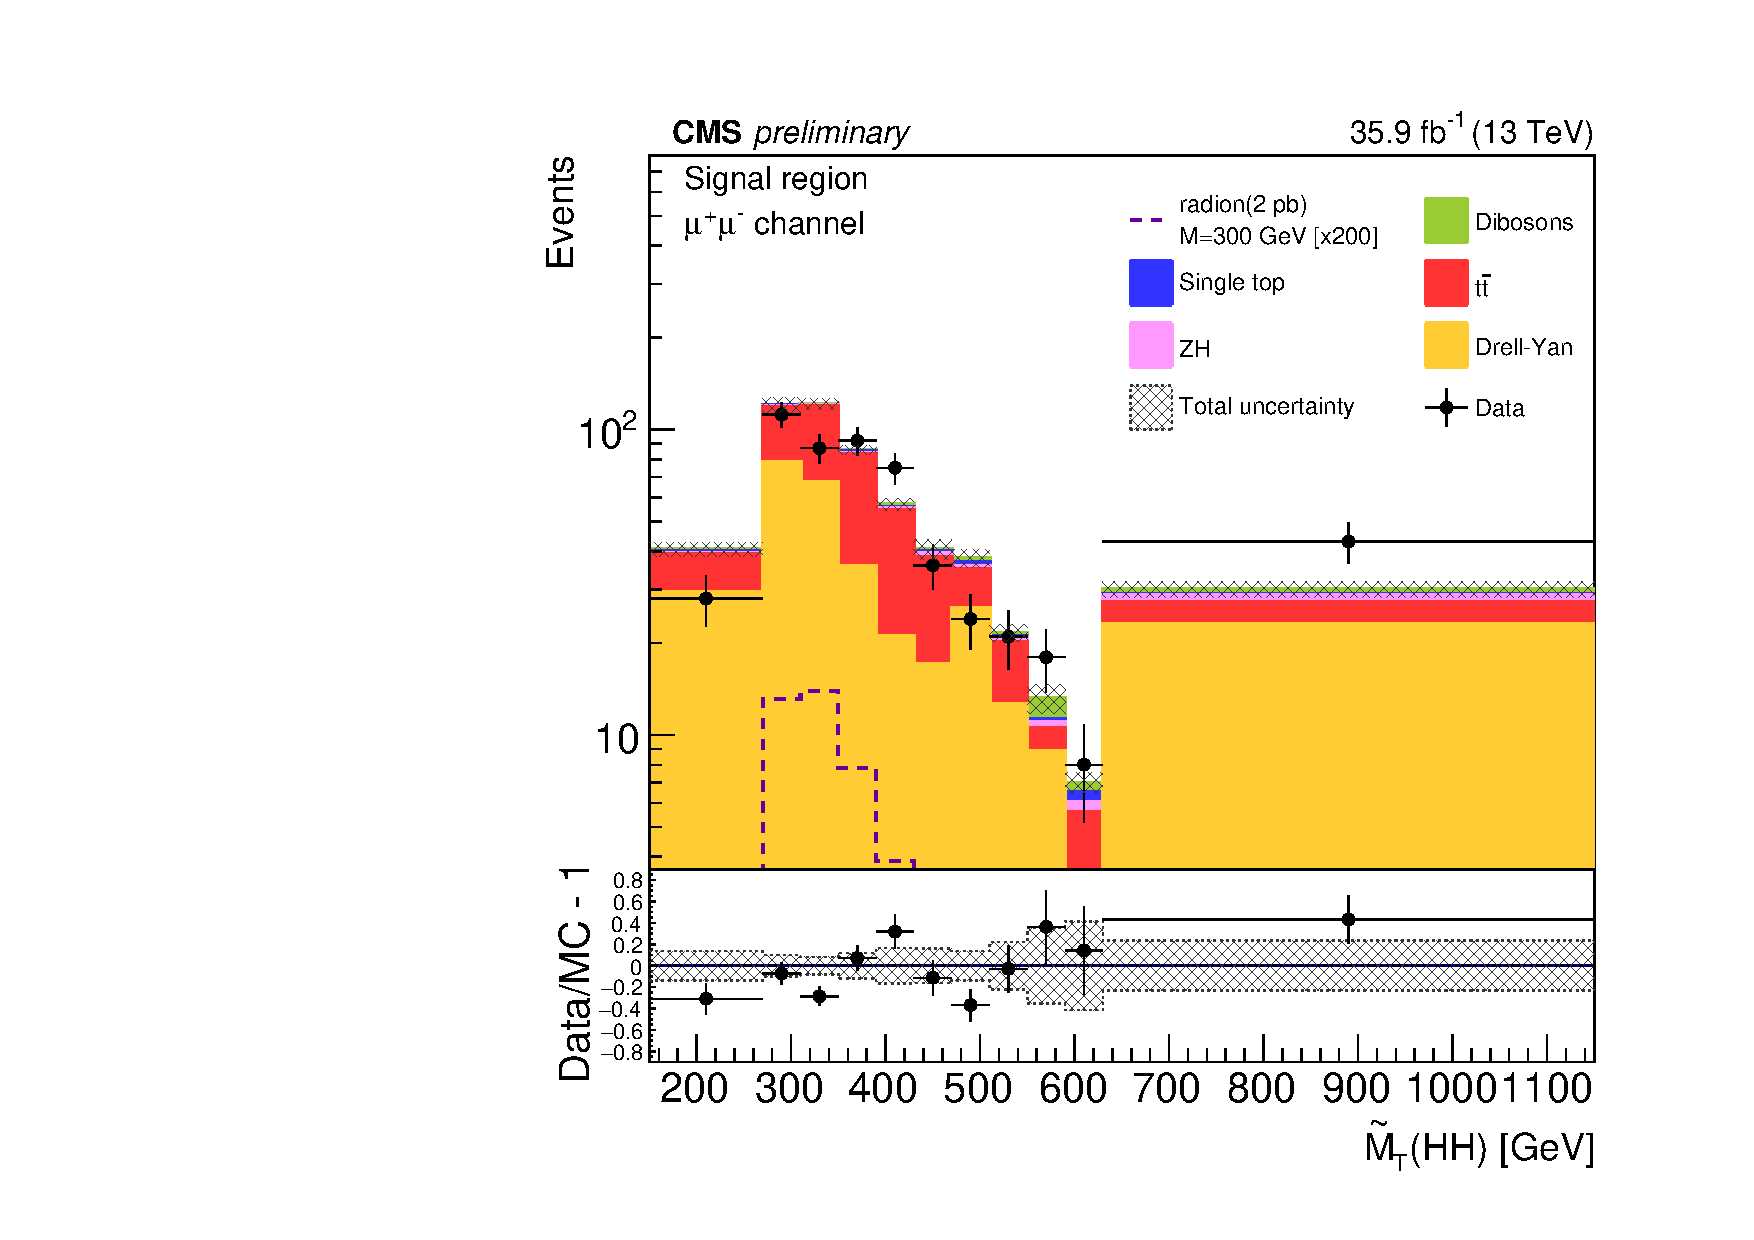
\includegraphics[width=0.31\textwidth]{hhMt_mm_SR_FullPostfit_plot_nov16_2_radion.pdf} \\
    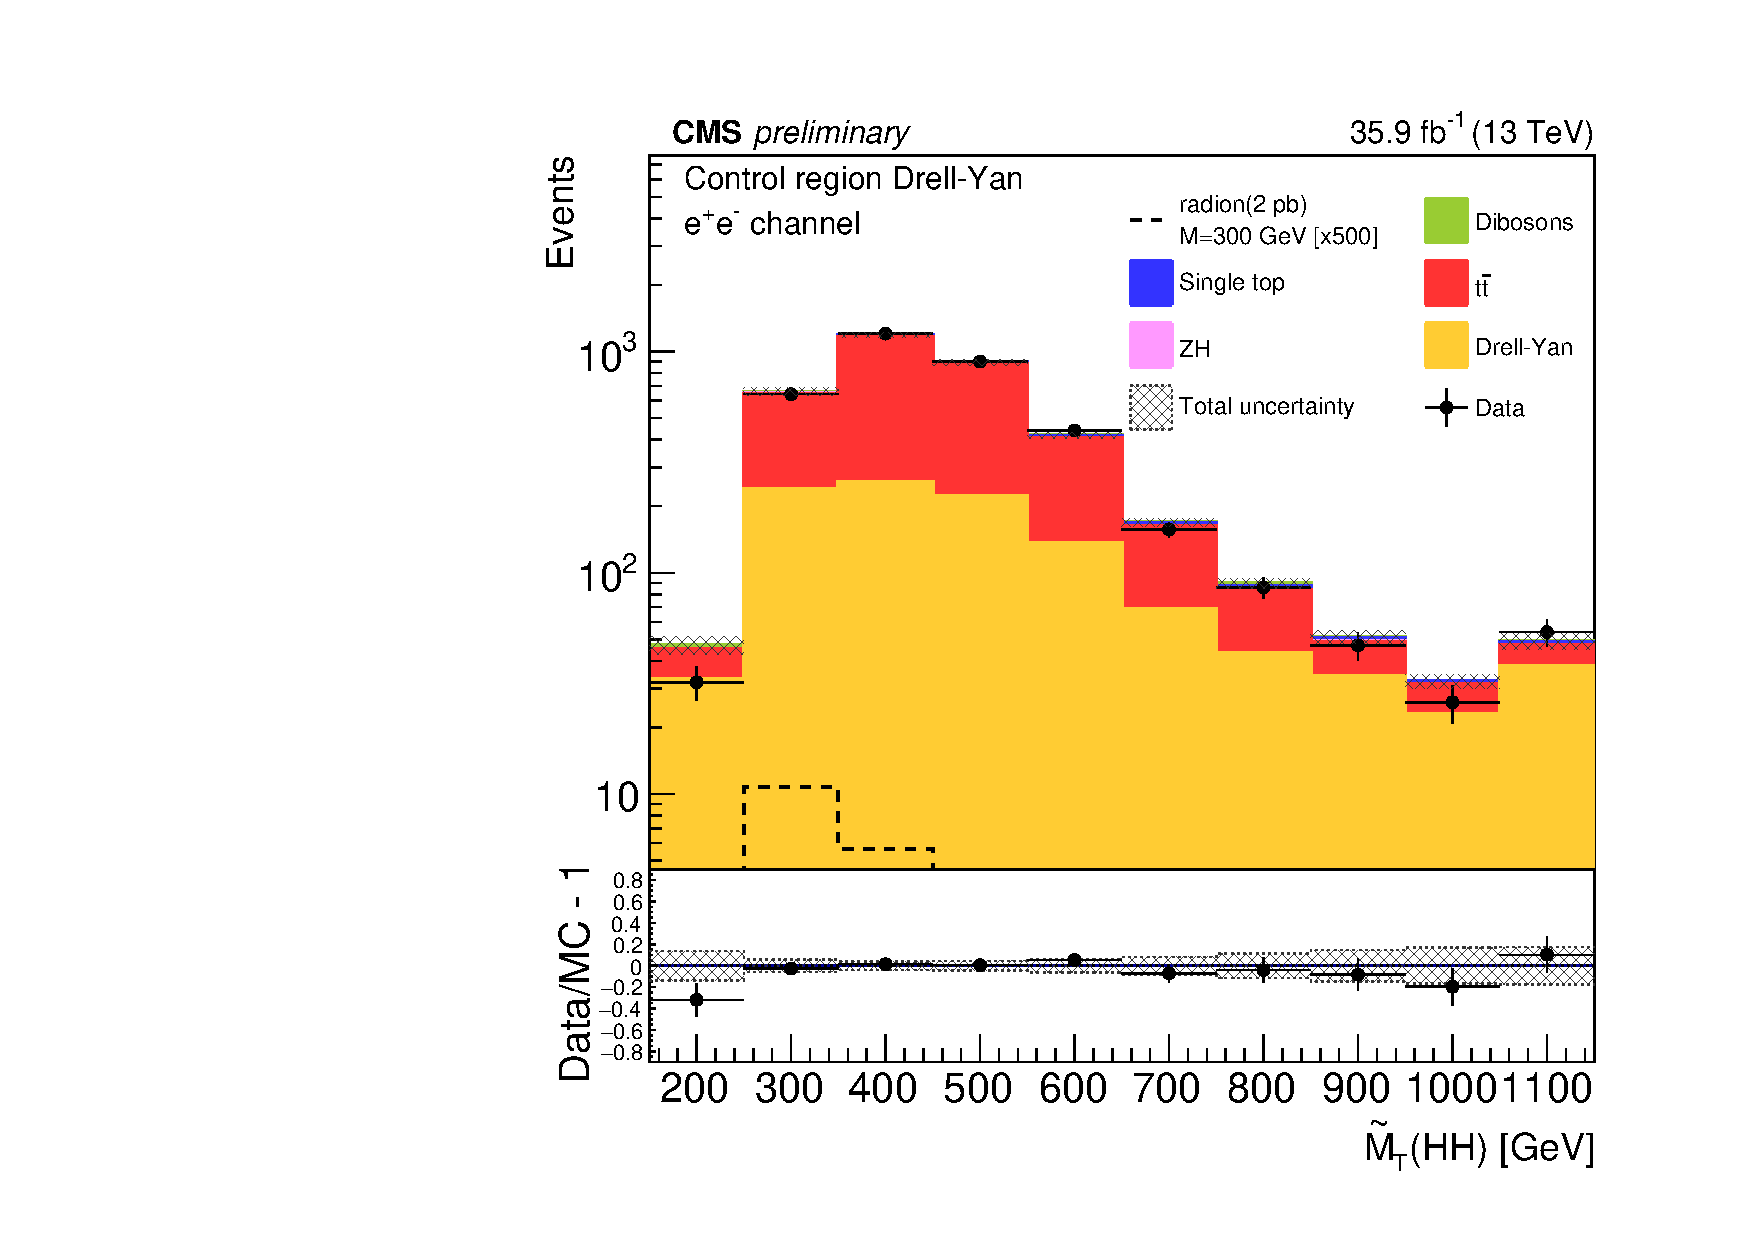
\includegraphics[width=0.31\textwidth]{hhMt_ee_CRDY_FullPostfit_plot_nov16_2_radion.pdf}
    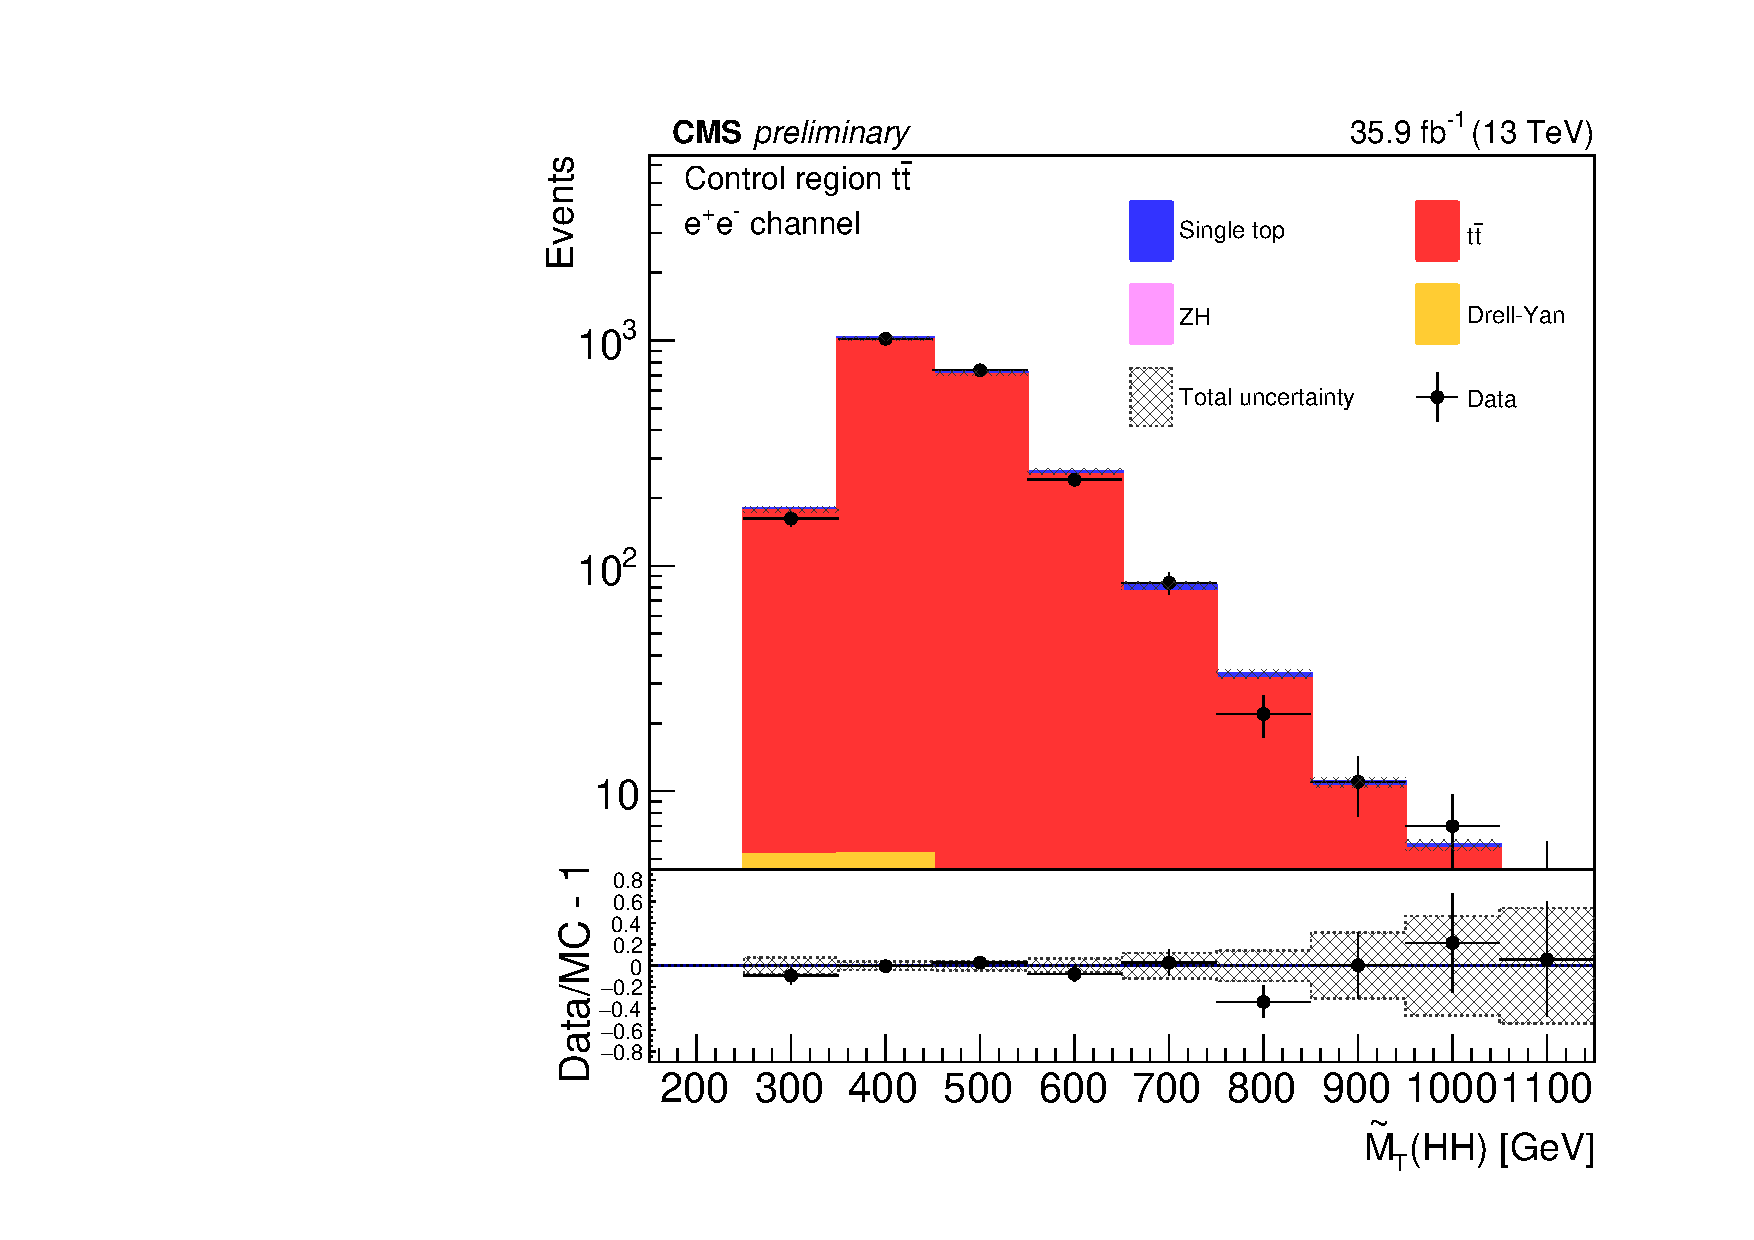
\includegraphics[width=0.31\textwidth]{hhMt_ee_CRTT_FullPostfit_plot_nov16_2_radion.pdf}
    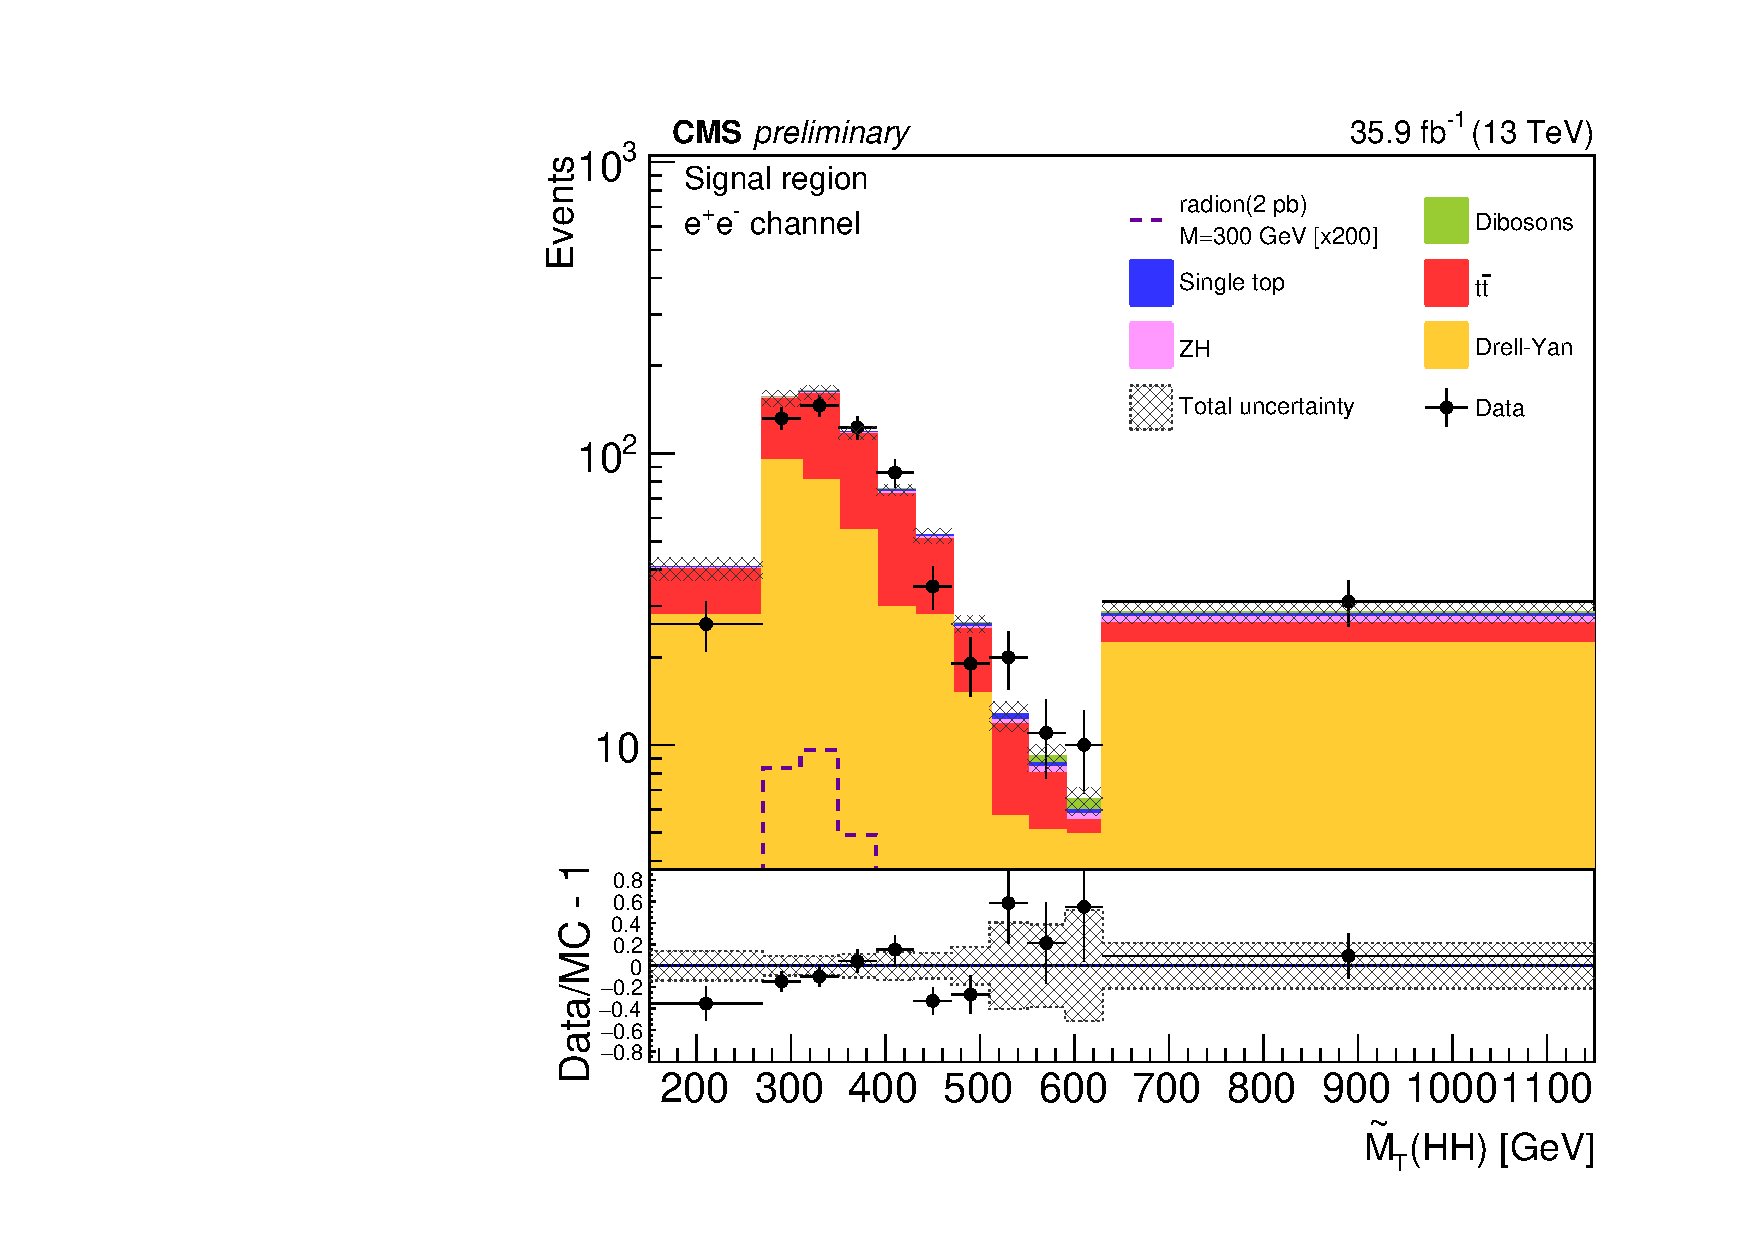
\includegraphics[width=0.31\textwidth]{hhMt_ee_SR_FullPostfit_plot_nov16_2_radion.pdf}
    \caption{Transverse mass of the reconstructed HH candidates for data, the simulated signal radion sample
    for the 300 GeV mass hypothesis, and simulated backgrounds scaled according to the fit results. The top
    row shows the figures for the muon channel while the bottom row is for the electron channel. For each row,
    the left plot is for the Drell-Yan control region, the middle is for the \ttbar control region, and the right
    is for the signal region. Signal normalization choice is discussed in the text. The crosshatched area represents
    the sum of statistical and systematic uncertainties.}
    \label{fig:MCcomparisons_radion}
%                                                                                                                 
% Comparison of data and simulation.  Transverse mass of                                                          
%      the reconstructed HH candidate for 300 GeV signal mass                                                     
%      hypothesis, electron channel. Left: Drell-Yan control region. Middle: \ttbar                               
%      control region. Right: signal region. }                                                                    
%    \label{MCcomparisons_electrons}                                                                              
  \end{center}
\end{figure}







\section{Scale Factors}
%\section{HLT Lepton Scale Factors}

Electron ID and ISO scale factors, as well as HLT scale factors (Fig.~\ref{fig:trigger_eff_diele}), have been computed by VHbb group, which ntuples and analysis setup we reutilise. Scale factors have been presented at the EGamma physics object groups (POG) meeting~\cite{egSF} and fully approved. We reuse those scale factors and apply them to our MC samples. 

Muon ID scale factors, as well as ISO scale factors, have been derived separately for runs G/H and B/C/D/E/F runs (2016 data at LHC has been split into several "runs") and then luminosity averaged to obtain the final numbers ~\cite{muonIDnISO}. Tracker scale factors (~\ref{fig:trigger_eff_diele}) are taken from the Muon POG twiki page~\cite{muonTRK} and used as is. HLT dimuon scale factors were derived by VHbb group and further approved by the muon POG. These scale factors were derived separately for run H (Fig.~\ref{fig:trigger_SF_dimu_H}) and B/C/D/E/F/G (Fig.~\ref{fig:trigger_SF_dimu_BCDEFG}) runs and then luminosity averaged ~\cite{muonTrigger}. On top, separate scale factors are calculated for the dZ requirement of HLT\_Mu17\_TrkIsoVVL\_Mu8\_TrkIsoVV\L\_DZ\_v* OR HLT\_Mu17\_TrkIsoVVL\_TkMu8\_TrkIsoVVL\_DZ\_v* triggers, using dilepton events that have already passed the HLT\_Mu17\_TrkIsoVVL\_Mu8\_TrkIsoVVL\_v* OR HLT\_Mu17\_TrkIsoVVL\_TkMu8\_TrkIsoVVL\_v* triggers (Fig. ~\ref{fig:trigger_SF_dimu_dZ_H}).

